%%%%%%%%%%%%%%%%%%%%%%%%%%%%%%%%%%%%%%%%%%%%%%%%%%%%%%%
%% Bachelor's & Master's Thesis Template             %%
%% Copyleft by Artur M. Brodzki & Piotr Woźniak      %%
%% Faculty of Electronics and Information Technology %%
%% Warsaw University of Technology, 2019-2020        %%
%%%%%%%%%%%%%%%%%%%%%%%%%%%%%%%%%%%%%%%%%%%%%%%%%%%%%%%

\documentclass[
    left=2.5cm,         % Sadly, generic margin parameter
    right=2.5cm,        % doesnt't work, as it is
    top=2.5cm,          % superseded by more specific
    bottom=3cm,         % left...bottom parameters.
    bindingoffset=6mm,  % Optional binding offset.
    nohyphenation=false % You may turn off hyphenation, if don't like.
]{src/wut-thesis}

\langpol % Dla języka angielskiego mamy \langeng
\graphicspath{{tex/img/}}             % Katalog z obrazkami.
\addbibresource{bibliografia.bib} % Plik .bib z bibliografią

\begin{document}

%--------------------------------------
% Strona tytułowa
%--------------------------------------
\MasterThesis % Dla pracy inżynierskiej mamy \EngineerThesis
\facultyeiti
\instytut{Informatyki}
\kierunek{informatyka}
\specjalnosc{Sztuczna inteligencja}
\title{Generowanie podpisów do obrazków}
\engtitle{Image caption generation}
\author{Kacper Kostecki}
\album{300236}
\promotor{dr inż. Piotr Andruszkiewicz}
\date{\the\year}
\maketitle

%--------------------------------------
% Streszczenie po polsku
%--------------------------------------
\cleardoublepage % Zaczynamy od nieparzystej strony
\abstract We wszelkich dziedzinach życia człowieka obrazy stanowią istotny element komunikacji i przekazu informacji, jednak człowiek napotyka trudności w efektywnym przetwarzaniu i wykorzystywaniu tej ogromnej ilości wizualnych danych. Analiza i interpretacja obrazów są zadaniem wymagającym znacznego nakładu czasu i wysiłku intelektualnego. Rozwiązaniem tego problemu są algorytmy uczenia maszynowego umożliwiające automatyczne generowanie podpisów do obrazów, co znacząco ułatwia cały proces wydobywania z nich informacji. Jednakże ich wykorzystanie generuje kolejną przeszkodę: zasoby komputerowe. W celu rozwiązania tak skomplikowanego problemu, jakim jest generowanie podpisów do obrazów, wykorzystane algorytmy są niezwykle skomplikowane, a co za tym idzie, potrzebują coraz większą ilość zasobów komputerowych. Celem niniejszej pracy dyplomowej było zbadanie skuteczności, jak również efektywności wykorzystywanych algorytmów do generowania podpisów do obrazków.
\keywords podpisy obrazków, język naturalny, wizja komputerowa, zasoby komputerowe

%--------------------------------------
% Streszczenie po angielsku
%--------------------------------------
\vspace{1cm}
\secondabstract In all areas of human life, images constitute an essential element of communication and information transmission, however, humans encounter difficulties in efficiently processing and utilizing this vast amount of visual data. Analyzing and interpreting images is a task that requires significant time and intellectual effort. Machine learning algorithms provide a solution to this problem by enabling automatic generation of captions for images, greatly facilitating the process of extracting information from them. However, their utilization presents another challenge: computer resources. To address the complex problem of generating captions for images, the employed algorithms are highly intricate, thus requiring increasingly larger amounts of computer resources. The aim of this thesis was to examine the effectiveness and efficiency of the utilized algorithms for generating captions for images.
\secondkeywords image captioning, natural language processing, computer vision, computer resources

%--------------------------------------
% Oświadczenie o autorstwie
%--------------------------------------
\cleardoublepage  % Zaczynamy od nieparzystej strony
\pagestyle{plain}
\makeauthorship

%--------------------------------------
% Spis treści
%--------------------------------------
\cleardoublepage % Zaczynamy od nieparzystej strony
\tableofcontents

%--------------------------------------
% Rozdziały
%--------------------------------------
\cleardoublepage % Zaczynamy od nieparzystej strony
\pagestyle{headings}

\newpage % Rozdziały zaczynamy od nowej strony.
\section{Wstęp}
W ostatnich latach, wraz z rozwojem technologii cyfrowej i internetu, liczba dostępnych obrazów, zdjęć i diagramów znacząco wzrosła. Zarówno w mediach społecznościowych, stronach internetowych, jak i w różnych obszarach działalności, takich jak medycyna, nauka czy przemysł, obrazy stanowią istotny element komunikacji i przekazu informacji. Jednak człowiek napotyka trudności w efektywnym przetwarzaniu i wykorzystywaniu tej ogromnej ilości wizualnych danych. Analiza i interpretacja obrazów są zadaniem wymagającym znacznego nakładu czasu i wysiłku intelektualnego. Człowiek musi poświęcić wiele uwagi i sił, aby opisać, co~przedstawia dany obraz, uwzględniając detale, kontekst, emocje czy inne istotne elementy. Ten proces może być jeszcze bardziej uciążliwy w przypadku dużych zbiorów wizualnych danych, gdzie manualne generowanie opisów staje się nieefektywne i czasochłonne. W odpowiedzi na te wyzwania, rozwój technik sztucznej inteligencji i uczenia maszynowego otwiera nowe perspektywy w automatycznym generowaniu podpisów do obrazków. Algorytmy uczenia maszynowego pozwalają na tworzenie modeli komputerowych, które są w stanie analizować obrazy, wyodrębniać z nich cechy, rozpoznawać obiekty i kontekst, a następnie generować opisy tekstowe na podstawie tej wiedzy. Dzięki temu automatyczne generowanie podpisów staje się realnym rozwiązaniem, które może przyspieszyć i ułatwić proces analizy obrazów. Oprócz oszczędności czasu i wysiłku, automatyczne generowanie podpisów do obrazków ma również potencjalne znaczenie dla osób niewidomych. Dla nich dostęp do informacji wizualnych jest ograniczony lub niemożliwy. Generowanie tekstowych opisów obrazów staje się zatem narzędziem, które umożliwia im lepsze zrozumienie i korzystanie z wizualnych treści. Dzięki automatycznym podpisom, osoby niewidome mogą otrzymać opisy obrazów, które pośrednio przekazują informacje wizualne, pozwalając im na lepszą orientację i uczestnictwo w kulturze wizualnej.
\subsection{Cel i motywacja pracy}
Celem niniejszej pracy było sprawdzenie skuteczności oraz efektywności aktualnych rozwiązań wykorzystywanych do automatycznego generowania opisów obrazów cyfrowych. Szczególna uwaga została zwrócona na poziom wykorzystywanych zasobów komputerowych w stosunku do poprawy samej skuteczności generowania opisów wraz z uwzględnieniem czasu treningowego. Narastającym problemem coraz bardziej rozwijających się algorytmów uczenia maszynowego jest ich rosnące zapotrzebowanie na zasoby komputerowe. Wraz z postępem w dziedzinie sztucznej inteligencji, modele oparte na głębokim uczeniu stają się coraz bardziej skomplikowane i wymagają większej mocy obliczeniowej oraz większych ilości danych treningowych. Jednym z głównych czynników wymagań zasobów komputerowych jest rozmiar i złożoność sieci neuronowych. Modele, takie jak splotowe sieci neuronowe czy rekurencyjne sieci neuronowe, mogą składać się z setek tysięcy lub nawet milionów parametrów. Trenowanie tych modeli wymaga dużych zbiorów danych oraz intensywnego obliczeniowo procesu optymalizacji tych parametrów. Kolejnym aspektem jest wykorzystanie sprzętu. W przypadku dużych i złożonych sieci neuronowych konieczne jest korzystanie z zaawansowanych jednostek przetwarzania graficznego lub specjalizowanych procesorów tensorowych, które są bardziej efektywne w wykonywaniu operacji macierzowych charakterystycznych dla uczenia maszynowego. Korzystanie z takiego specjalistycznego sprzętu może stanowić wyzwanie ze względu na wysokie koszty i dostępność. Ponadto w samych publikacjach dotyczących proponowanych rozwiązań często nie ma zawartych informacji o efektywności architektury w kontekście zasobów komputerowych.
         % Wygodnie jest trzymać każdy rozdział w osobnym pliku.
\newpage
\section{Teoria uczenia maszynowego}
Informatyka z dnia na dzień, coraz śmielej wkracza we wszelkie dziedziny życia człowieka. Dzięki jej rozwojowi wiele żmudnych, uciążliwych, czy też niebezpiecznych prac wykonywanych przez człowieka może zostać zautomatyzowane. Szczególny wkład w ten gwałtowny rozwój ma konkretna dziedzina informatyki: sztuczna inteligencja. Pozwala ona na rozwiązywanie skomplikowanych zadań takich jak przetwarzanie obrazów cyfrowych, czy też analiza języka naturalnego. Ze względu na dużą ilość informacji konieczną do przetworzenia, która zawarta jest, czy to w obrazach, czy w tekstach pisanych przez człowieka oraz ogromną różnorodność tychże danych, niezwykle problematyczne jest sformułowanie uniwersalnych algorytmów, które podjęłyby rozwiązanie problemów, jak na przykład lokalizacja obiektów w obrazach, czy ustalenie semantyki danego zdania. Z pomocą przychodzą tutaj algorytmy uczenia maszynowego należące do rodziny algorytmów sztucznej inteligencji. Pozwalają one przy pomocy uniwersalnego podejścia sformułować rozwiązanie danego problemu na podstawie historycznych danych.
\subsection{Sieci neuronowe}
Szczególnym rodzajem algorytmów uczenia maszynowego są sieci neuronowe. Zostały one stworzone na wzór neuronów obecnych w ludzkich organizmach. Składają się one z neuronów, które przetwarzają dane i przekazują do kolejnych neuronów razem tworzących warstwy. Każdy neuron posiada wagę, która jest ustalana w wyniku trenowania całej sieci przy pomocy danych dotyczących aktualnego problemu. Tak jak w przypadku ludzkiego mózgu, neurony w sieciach można komponować na wiele sposób. Do różnego rodzaju dziedzin, stosowane są różnego rodzaju architektury odpowiednio dostosowane do problemów z nimi związanych.
\subsection{Przetwarzanie języka naturalnego}
W celu przetwarzania języka naturalnego ogromną popularnością cieszą się algorytmy uczenia maszynowego, a w szczególności rekurencyjne sieci neuronowe. Ze względu na naturę języka ludzkiego, pojedyncze słowa najczęściej nie niosą ze sobą całości przekazywanych informacji -- konieczne jest wzięcie pod uwagę również kontekstu zdania, czy nawet całego tekstu. Taką możliwość dają rekurencyjne sieci neuronowe \cite{rnn}. Przy ich pomocy dane wejściowe przetwarzane są w postaci szeregu, a informacja dotycząca poprzedniego elementu jest uwzględniania przy przetwarzaniu następnego elementu. Umożliwia to również nieograniczanie długości przetwarzanych danych -- możliwe jest przetwarzanie kilku wyrazowych tekstów lub całych książek przy użyciu tej samej architektury sieci neuronowej. Schemat architektury sieci neuronowej został przedstawiony na rysunku \ref{fig:schemat-rnn}. Rekurencyjna sieć neuronowa była jednym z pierwszych takich rozwiązań oraz jednym z najpopularniejszych wykorzystywanych przy przetwarzaniu języka naturalnego. Przy jej pomocy można rozwiązać skutecznie wiele zadań, jednakże nie jest wolna od wad. Największym problemem z nią związanym jest duża niestabilność objawiająca się poprzez eksplozję lub zanikanie gradientu. Spowodowane jest to tym, iż w obliczeniach sieci rekurencyjnej za każdym razem uwzględniane są wyniki z poprzedniego przetworzenia. W przypadku chęci przetwarzania długich tekstów, mnożenie kolejnych wartości gwałtownie zwiększa lub zmniejsza wartość gradientu, co znacząco zaburza ostateczny wynik (przykładowo wartość 1,01 podniesiona do tysięcznej potęgi daje wynik ponad 10 tysięcy). W celu zaadresowania tychże problemów powstały rozszerzenia sieci rekurencyjnej. Najpopularniejsze z nich to: Long Short-term Memory \cite{lstm} oraz Gated Reccurent Unit \cite{gru}. Dzięki skomplikowaniu obliczeń oraz przekazywania danych w postaci kontekstu do kolejnych elementów szeregu, zjawisko eksplozji/zanikania gradientu nie ma tak znaczącego wpływu na ostateczne rezultaty.
\begin{figure}[!h]
  \centering
  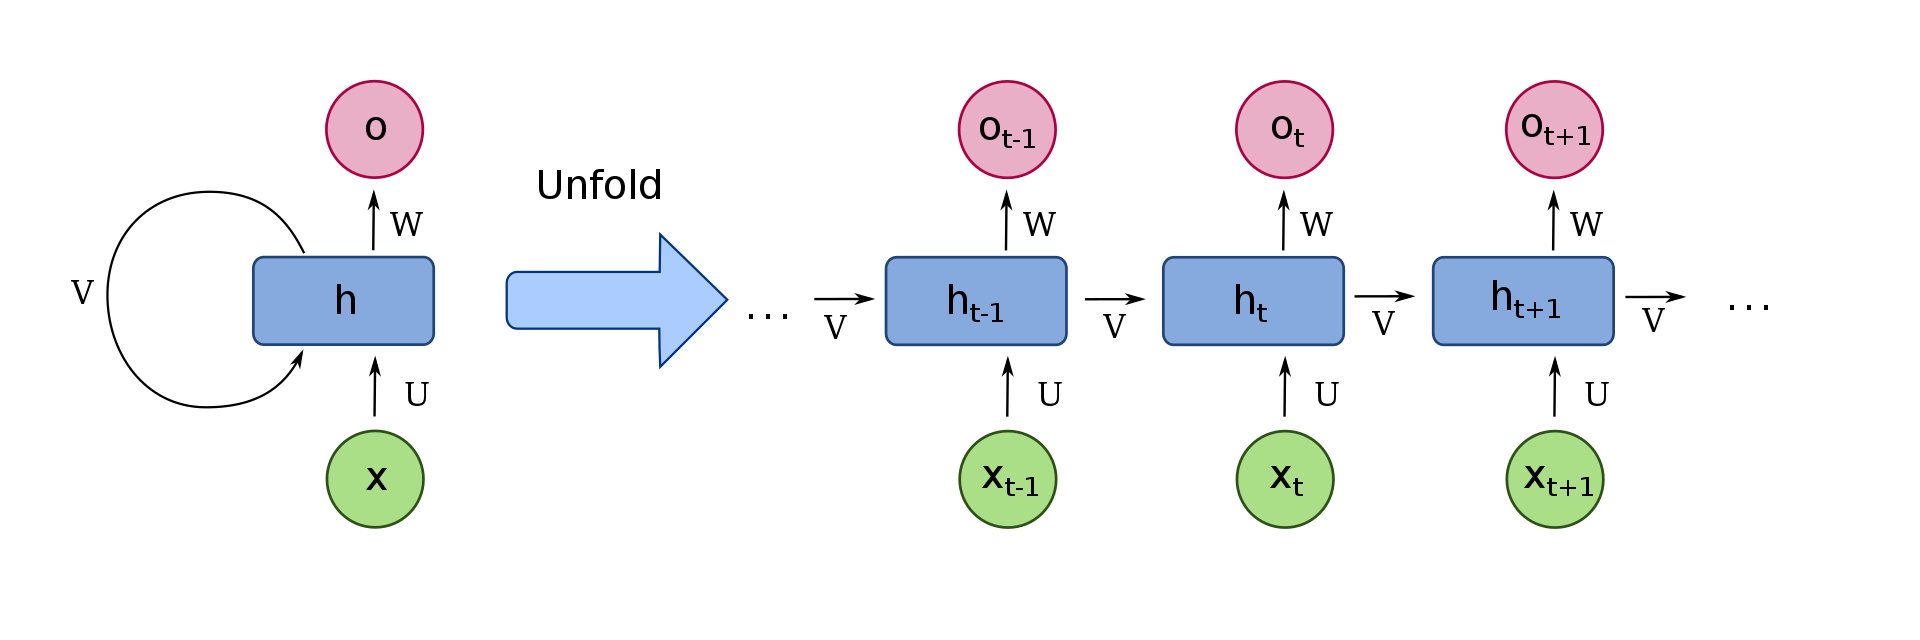
\includegraphics[width=.9\linewidth]{schemat-rnn}
  \caption{Architektura rekurencyjnej sieci neuronowej. Źródło: \cite{WikipediaEN:RNN}}
  \label{fig:schemat-rnn}
\end{figure}
\subsection{Atencja}
Atencja to kluczowy mechanizm w dziedzinie sieci neuronowych, który umożliwia modelom uczenia maszynowego skupienie się na odpowiednich częściach danych wejściowych. Jest to szczególnie przydatne w przypadku analizy sekwencji, takich jak tłumaczenie maszynowe, rozpoznawanie mowy, generowanie tekstu itp.

Idea atencji opiera się na tym, że każda część danych wejściowych może mieć różne znaczenie dla wyniku końcowego. Zamiast traktować całą sekwencję jako jedną całość, atencja pozwala modelowi skupić się na istotnych fragmentach danych wejściowych w zależności od kontekstu.

W praktyce, atencja jest zazwyczaj implementowana jako dodatkowy moduł w sieci neuronowej. Moduł ten oblicza wagi dla poszczególnych części danych wejściowych, które określają, jak bardzo te części powinny być brane pod uwagę przy generowaniu wyniku. Wagi te są obliczane na podstawie podobieństwa między danymi wejściowymi a aktualnym stanem modelu.
\subsection{Wstępne przetwarzanie danych}
W celu przygotowania danych do przetwarzania przez sieci neuronowe konieczne jest ich odpowiednie ujednolicenie oraz przetworzenie do postaci jak najlepiej przyjaznej dla komputera. Obrazy cyfrowe nie wymagają specjalnego przetwarzania, ponieważ są już w postaci macierzy zawierających dane poszczególnych pikseli w postaci kodów RGB -- wystarczającym jest znormalizowanie ich wartości oraz ujednolicenie ich wymiarów w celu uproszczenia obliczeń. W przypadku wartości tekstowych, które mają być wartością wyjściową całej architektury, przetworzenie ich do formy zrozumiałej przez komputer jest znacznie bardziej utrudnione. Ma na to wpływ duża złożoność języków naturalnych jak na przykład różna długość słów, różne końcówki wyrazów, które niekoniecznie mają wpływ na samo znaczenie słowa. W celu ujednolicenia tychże rozbieżności tworzony jest słownik, w którym każde słowo posiada odpowiedni indeks w postaci liczby -- w takiej postaci komputer jest w stanie operować na liczbach, a w momencie potrzeby otrzymania danych w postaci tekstu w języku naturalnym, wystarczy zamienić indeksy z odpowiadającymi im słowami.
\subsection{Wizja komputerowa}
Przetwarzanie wszelkiego rodzaju obrazów cyfrowych w postaci zdjęć filmów itd. jest niezwykle problematyczne, ponieważ pojedyncze zdjęcie wykonane w jakości HD posiada prawie milion pikseli. Dodatkowo biorąc pod uwagę wiele kombinacji, w których zdjęcie może być wykonane, dane konieczne do przetworzenia oraz sformułowanie na ich podstawie algorytmów rozwiązujących dużą część problemów z nimi związanych jest praktycznie niemożliwe. Z tychże względów ogromną popularnością wśród rozwiązywania problemów związanych z wizją komputerową cieszą się algorytmy uczenia maszynowego, a w szczególności splotowe sieci neuronowe. Charakteryzują się one różnymi rodzajami warstw. Do podstawowych typów warstw należą:
\begin{itemize}
  \item warstwa splotowa -- jest to podstawowa warstwa, która składa się z zestawu filtrów splotowych wykorzystujących operację splotu. Filtry te przesuwają się po obrazie wejściowym i wykrywają w nim wzorce o różnym stopniu skomplikowania.
  \item Warstwa aktywacji -- wyniki operacji splotu są przetwarzane za pomocą funkcji aktywacji, takiej jak tangens hiperboliczny, co pozwala na generowanie tak zwanych map cech dla każdego filtra z warstwy splotowej.
  \item Warstwa grupująca -- rozmiar otrzymanych map cech wygenerowanych przez warstwę splotową jest redukowany poprzez grupowanie wartości w oknie i zastępowanie ich pojedynczą wartością reprezentującą cechy w danym obszarze. Najczęściej stosowane są dwa rodzaje operacji grupujących: max-pooling i average-pooling.
\end{itemize}
Powyższe warstwy najczęściej występują wielokrotnie w obrębie jednej sieci, co pozwala na wydobywanie wzorców z przetwarzanego obrazu na różnym poziomie kontekstu. Dalsze przetwarzanie oraz grupowanie map cech obrazu daje możliwość uwzględnienia szerszego kontekstu, jaki jest zawarty w obrazie niż jedynie w obrębie najbliższego sąsiedztwa danego piksela. Schemat podstawowej architektury splotowej sieci neuronowej służącej do klasyfikacji obrazu został przedstawiony na rysunku \ref{fig:schemat-cnn}.
\begin{figure}[!h]
  \centering
  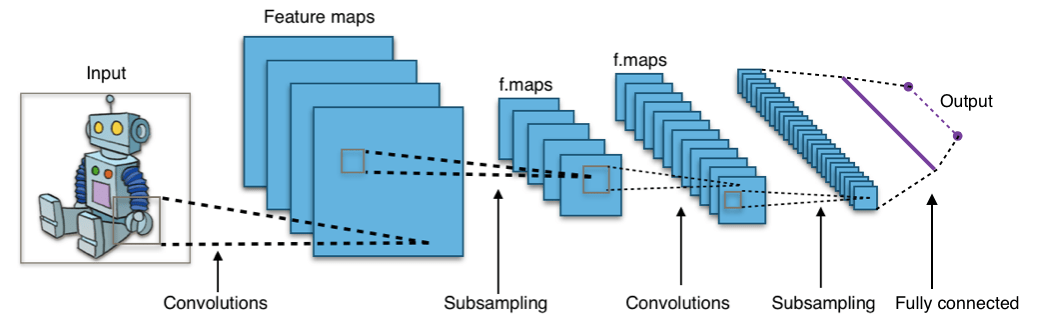
\includegraphics[width=.9\linewidth]{schemat-cnn}
  \caption{Architektura splotowej sieci neuronowej. Źródło: \cite{WikipediaEN:CNN}}
  \label{fig:schemat-cnn}
\end{figure}

\newpage % Rozdziały zaczynamy od nowej strony.
\section{Generowanie podpisów do obrazów -- aktualne rozwiązania}
W celu wygenerowania podpisu do obrazu przy użyciu algorytmów uczenia maszynowego wykorzystuje się sieci neuronowe. Sam proces generowania podpisów można rozbić na dwa etapy: przetwarzanie obrazu oraz generowanie tekstu. Z tego względu najpopularniejsze podejścia wykorzystują połączenia sieci wykorzystywanych do przetwarzania obrazów wraz z sieciami wykorzystywanymi do przetwarzania języka naturalnego. Takie podejście wyodrębnia dwa główne moduły w całej architekturze sieci:
\begin{itemize}
  \item moduł kodujący obraz -- jego danymi wejściowymi jest obraz w postaci macierzy pikseli, natomiast wyjściem jest wektor sprowadzony do postaci zgodnej z formatem wejściowym modułu dekodującego,
  \item moduł dekodujący zakodowany obraz wcześniej obraz -- wejściem tego modułu jest wyjście modułu kodującego, natomiast wyjściem jest ostatecznie wygenerowane zdanie.
\end{itemize}
\begin{figure}[H]
  \centering
  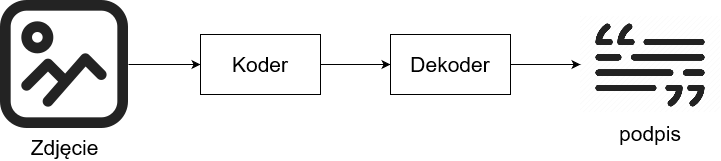
\includegraphics[width=.9\linewidth]{diagram}
  \caption{Typowa architektura generatora podpisów. Opracowanie własne}
  \label{fig:schemat-captioning}
\end{figure}
\subsection{Moduły kodujące}
Ze względu na niezwykle dużą skuteczność, jak również popularność, najczęściej wykorzystywaną siecią neuronową jako moduł kodujący jest splotowa sieć neuronowa. Główną jej modyfikacją, w celu dostosowania do problemu, jakim jest generowanie podpisów, jest dopasowanie ostatnich warstw w taki sposób, aby~ostateczny wektor wyjściowy był kompatybilny z typowym formatem danych wejściowych sieci wykorzystywanych w dziedzinie przetwarzania języka naturalnego.
\subsubsection{Bardzo głębokie sieci splotowe}
Jednym z częściej wykorzystywanych rodzajów sieci splotowej są głębokie sieci neuronowe. Charakteryzują się one dużą liczbą warstw splotowych oraz małymi wielkościami filtrów. Aktualnie istnieje wiele architektur wykorzystujących takie podejście. Jedną z pierwszych była sieć VGGNet \cite{vggnet}. Dzięki zastosowaniu dużej liczby warstw splotowych możliwe było klasyfikowanie obrazów o dużej rozdzielczości z bardzo wysoką skutecznością. Dużym minusem tego rodzaju sieci są wymagane zasoby. Ze względu na dużą ilość warstw konieczna jest alokacja duże ilości pamięci w jednostce GPU, a samo przetworzenie danych przez sieć wymaga wielu obliczeń.
\subsubsection{Transformer wizyjny}
Transformer wizyjny \cite{vit} to model przetwarzania obrazów, który różni się od tradycyjnych architektur zawierających sieci splotowe. Opiera się on na transformerze znanym głównie z zastosowań w przetwarzaniu języka naturalnego. Przy jego pomocy obraz jest przetwarzany poprzez podzielenie na nienachodzące się bloki, a każdy blok reprezentowany jest jako token, podobnie jak słowa w zdaniu. Te tokeny są traktowane jako sekwencja wejściowa dla modelu transformera. Poglądowy diagram przedstawiający architekturę transformera wizyjnego został przedstawiony na rysunku \ref{fig:vit-architecture}.
\begin{figure}[H]
  \centering
  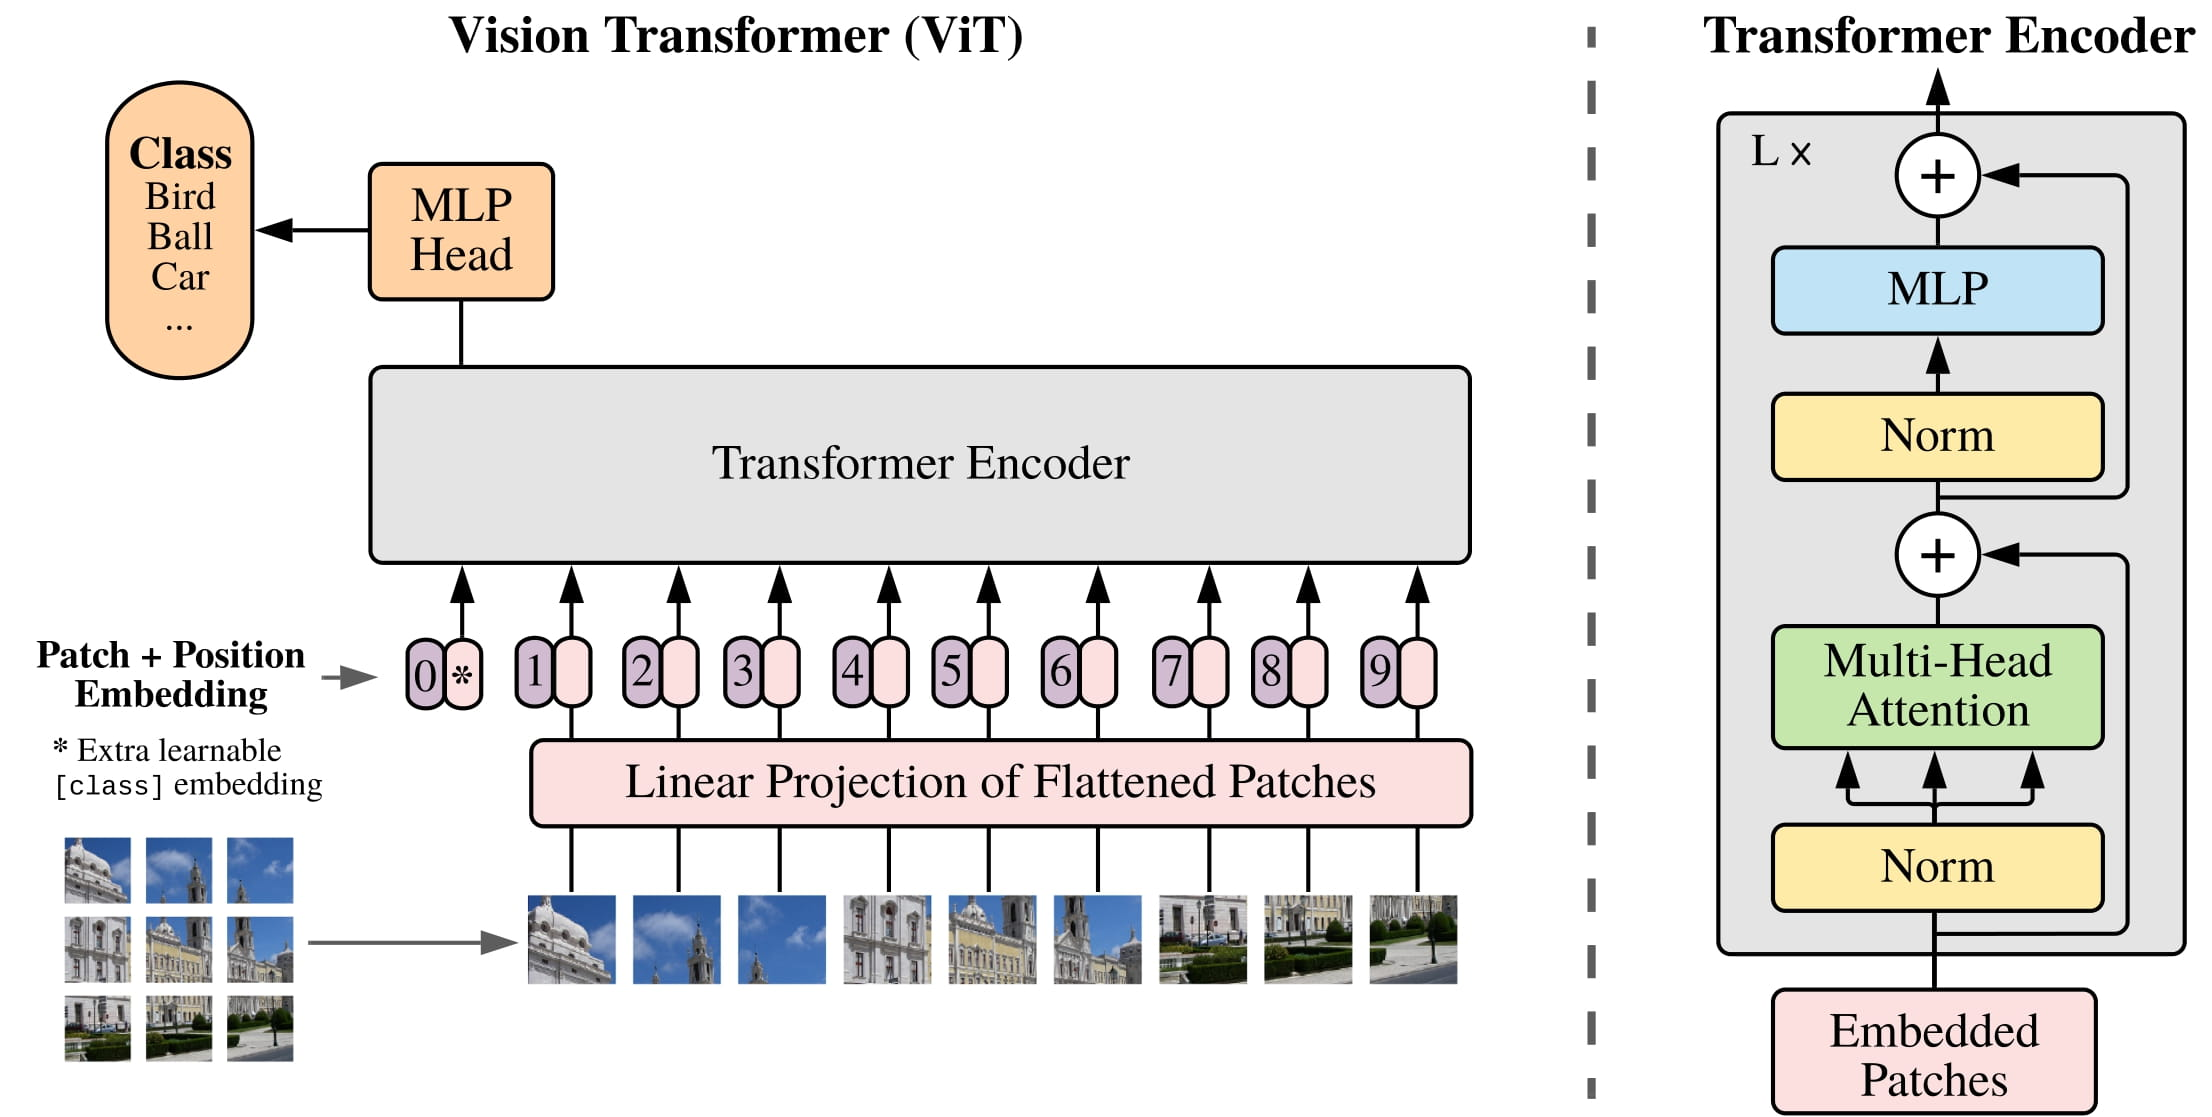
\includegraphics[width=.95\linewidth]{vit_architecture}
  \caption{Diagram architektury transformera wizyjnego. Źródło: \cite{vit}}
  \label{fig:vit-architecture}
\end{figure}
\noindent Dane wyjściowe z kodera transformera przetwarzane są w bardzo podobny sposób jak w przypadku danych wyjściowych głębokich warstw sieci splotowych -- przy pomocy w pełni połączonych warstw, wektor wyjściowy jest sprowadzany do postaci wektora zawierającego odpowiednie klasy, co zostało przedstawione na diagramie przy pomocy bloku ,,MLP Head'' oraz ,,Class''.
\subsection{Moduły dekodujące}
Dzięki sprowadzeniu obrazu do formatu zwykłego wektora poprzez moduł kodujący możliwe jest wykorzystanie większości rozwiązań dedykowanych do zwykłych zadań przetwarzania języka naturalnego. Jako analogiczną dziedzinę można tutaj wyróżnić zagadnienie związane z generowaniem odpowiedzi na pytania -- główną różnicą w przypadku generowania podpisów jest sprowadzenie obrazu do wartości możliwe do przetworzenia przez moduł kodujący. W przypadku zagadnień związanych z generowaniem odpowiedzi, przetwarzany jest tekst, natomiast w przypadku generowania podpisów są to obrazu. Dalsza część architektury, czyli moduł kodujący, jest analogiczna w obu przypadkach. Częstym wyborem jest podstawowa rekurencyjna sieć neuronowa. W przypadku takiej sieci wektor będący wyjściem modułu kodującego służy jako pierwszy element wejściowy moduły dekodującego. Naturalnie możliwe jest wykorzystywanie bardziej zaawansowanych odmian sieci rekurencyjnej jak LSTM oraz GRU. Również wykorzystywane są moduły atencji, w których przypadku szczególnie użyteczne są głębokie sieci neuronowe. Wyniki z poprzednich warstw splotowych służą jako kontekst, z którego może korzystać moduł atencji.
\subsubsection{Transformer}
% MAYBE rozwinąć
Tak jak w przypadku pozostałych problemów związanych z przetwarzaniem języka naturalnego, również w kontekście generowania podpisów do obrazów, popularnością cieszy się sieć Transformer \cite{transformer}. Główną różnicą w porównaniu do klasycznych sieci rekurencyjnych jest przetwarzanie przez transformer sekwencji w całości, a nie pojedynczych jej elementów. Takie działanie jest możliwe dzięki zastosowaniu modułu atencji oraz zakodowania pozycyjnego, czyli dodania informacji o pozycji elementu w sekwencji do jego wartości. Sama atencja pozwala na określenie znaczenia danych elementów sekwencji w kontekście jej całości. Jest to znacząca przewaga nad sieciami rekurencyjnymi, które biorą pod uwagę jedynie aktualnie przetwarzany element oraz dane wygenerowane na podstawie wszystkich wcześniej przetworzonych elementów. Wykorzystanie tych rozwiązań również niweluje całkowicie problem eksplozji lub zanikania gradientu, który występuje w przypadku sieci rekurencyjnych.
\subsection{Przykład architektur}
Architektura NIC (ang. Neural Image Caption) \cite{nic} wykorzystuje połączenie splotowej sieci neuronowej oraz sieć LSTM, w celu generowania podpisów. Osiąga ona wartość BLEU-4 na poziomie 27,7 dla zbioru MS COCO \cite{mscoco}.

Bardziej rozbudowana architektura GIT (ang. Generative Image-to-text Transformer) \cite{wang2022git} na zbiorze danych MS COCO osiągnęła wartość metryki BLEU-4 równą 43,2 -- wynik o 50\% lepszy. Wykorzystuje ona model Transformera wizyjnego jako moduł kodujący wraz z klasycznym Transformerem wykorzystanym jako moduł dekodujący. Rozwiązanie to pochodzi z 2022 roku i aktualnie osiąga jedne z najlepszych wyników w dziedzinie generowania podpisów do obrazków.

Architektura OFA (ang. Once for all) \cite{wang2022ofa} została stworzona z myślą o wielozadaniowości, dzięki czemu jest w stanie rozwiązać wiele zadań związanych z przetwarzaniem obrazów cyfrowych, w tym generowania podpisów. Model ten nie jest ograniczony jedynie do przetwarzania obrazów, ponieważ opiera się on na metodzie seq2seq, polegającej na przetwarzanie pewnej sekwencji do innej sekwencji. Jego danymi wejściowymi są dane językowy, którym może towarzyszyć obraz, z tego względu oprócz macierzy pikseli danego obrazka konieczne również jest podanie tekstu w postaci formuły informującej architekturę o konieczności wygenerowania podpisu jak na przykład „co opisuje obraz?”. Wszelkie typy zadań rozwiązywane przez architekturę OFA zostały zobrazowane na rysunku \ref{fig:ofa-tasks} stworzonym przez autorów sieci.
\begin{figure}[H]
  \centering
  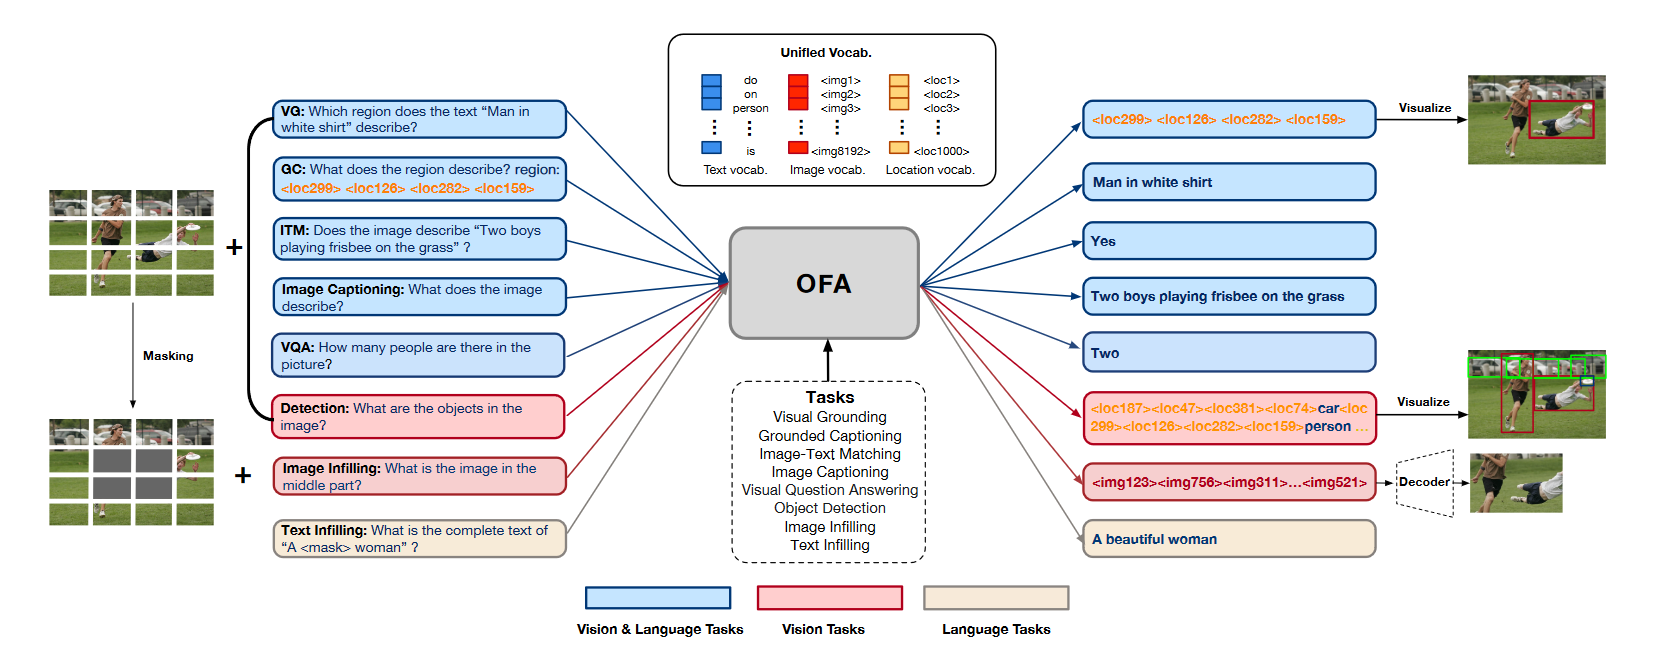
\includegraphics[width=\linewidth]{ofa_tasks}
  \caption{Diagram przedstawiający możliwe typy zadań rozwiązywane przez architekturę OFA. Źródło: \cite{wang2022ofa}}
  \label{fig:ofa-tasks}
\end{figure}
% MAYBE opisać technikalia architektury OFA 
\subsection{Wydajność aktualnych rozwiązań}
Publikowanych jest coraz więcej artykułów dotyczących uczenia maszynowego, jednakże ciężko jest znaleźć publikacje podejmujące problem, jakim są wysokie wymagania sprzętowe potrzebne do stworzenia takiego rozwiązania, jak również jego wykorzystywania. Najczęściej w przypadku opisywania autorskiej architektury sieci neuronowej, autorzy podają ramy czasowe poświęcone na trenowanie architektury wraz z nazwą wykorzystywanej jednostki GPU. O wiele rzadziej pojawia się informacja o samym czasie potrzebnym do przetworzenia pojedynczej wartości wejściowej w kontekście późniejszego wykorzystywania proponowanego rozwiązania.
Przykładem publikacji, które poruszają problem wysokich wymagań sprzętowych rozwiązań dotyczących neuronowych sieci splotowych oraz rekurencyjnych są:
\begin{itemize}
  \item Analiza wydajności splotowych sieci neuronowych bazujących na GPU \cite{cnn-compare},
  \item Optymalizacja wydajności rekurencyjnych sieci neuronowych wykorzystujących GPU \cite{rnn-compare}.
\end{itemize}
Niestety ze względu na o wiele mniejszą popularność dziedziny generowania podpisów do obrazków, ciężko znaleźć badania dotyczące konkretnie tego problemu. W łatwy sposób można oszacować, w jakich proporcjach zmieniać będzie się sama wydajność wykorzystywanych architektur poprzez połączenie czasów jednego modułu wraz z czasami drugiego modułu otrzymanymi z istniejących badaniach. Mimo wszystko takich wyników nie można uznać za dokładne ze względu na konieczność wprowadzenia modyfikacji w konkretnych architekturach modułów, jak również zupełnie różne środowiska testowe wykorzystywane w konkretnych badaniach. Dodatkowym problemem jest brak informacji o skuteczności danej architektur w kontekście zastosowanych zasobów, co jest niezwykle istotnym aspektem, ponieważ w przypadku osiągnięcie niezwykle wydajnej architektury jednocześnie może ona osiągać o wiele słabszą dokładność generowanych wyników.

\newpage % Rozdziały zaczynamy od nowej strony.

\section{Opis przeprowadzonych eksperymentów}
W celu generowania podpisów do obrazków wykorzystana została architektura składającą się z modułu kodującego oraz modułu dekodującego. W eksperymentach zostały wykorzystane ich różne konfiguracje. Dodatkowo wyniki zostały porównane z architekturami dedykowanymi do zadania generowania podpisów.
\subsection{Wykorzystanie wstępnie wytrenowanych modeli}
Szeroką popularnością w dziedzinie trenowania modeli sieci neuronowych cieszy się technika przenoszenia wiedzy. Jest to technika uczenia maszynowego, w której model uczony jest na jednym zadaniu, a następnie wykorzystuje tę wiedzę do lepszego rozwiązania innego, zazwyczaj podobnego zadania. Może zostać ona podzielona na dwa kluczowe kroki:
\begin{itemize}
    \item Początkowe uczenie modelu na dużym zbiorze danych i zadaniu, na którym jest dostępna duża ilość informacji.
    \item  Dostosowanie modelu do nowego zadania. Parametry modelu są dostosowywane do specyfiki nowego zadania, a wagi nauczone podczas początkowe uczenia są używane jako punkt wyjścia.
\end{itemize}
W przypadku generowania podpisów do obrazków technikę przenoszenia wiedzy można zastosować poprzez wykorzystanie wcześniej wyuczonych modeli sieci splotowych w ramach modułu kodującego. Trenowanie splotowych sieci neuronowych od zera na dużym zbiorze danych może być czasochłonne i wymagać dużej ilości zasobów obliczeniowych. Wykorzystanie wstępnie wytrenowanych modeli pozwala uniknąć tego procesu, ponieważ modele te są już przeszkolone do ekstrakcji cech, co jest ich głównym zadaniem w całej architekturze. Z tego względu dane treningowe zostały poddane wcześniejszemu przetworzeniu przez moduł kodujący, a trening polegał na uczeniu jedynie modułu dekodującego. Wykorzystane moduły kodujące:
\begin{itemize}
    \item AlexNet \cite{alexnet} -- jedna z najbardziej wpływowych sieci w historii przetwarzania obrazów, cechuje ją duża liczba parametrów, co pozwala na wyodrębnienie dużej liczby cech.
    \item GoogLeNet \cite{googlenet} -- sieć charakteryzuje się modułami inception mającymi na celu efektywne wykorzystanie zasobów obliczeniowych.
    \item VGGNet \cite{vggnet} -- bardzo głęboka sieć neuronowa wykorzystująca małe filtry splotowe pozwalających na wyodrębnienie cech o różnym stopniu skomplikowania.
    \item ResNet \cite{resnet} -- bardzo głęboka sieć neuronowa charakteryzująca się blokami rezydualnymi, które umożliwiają efektywne uczenie się sieci neuronowej o dużej liczbie warstw.
    \item VIT \cite{vit} - transformer wizyjny będący rozszerzeniem modelu transformer. Implementuje on mechanizm atencji, w celu wyodrębniania poszczególnych cech obrazu.
\end{itemize}
Ze względu na wykorzystanie wstępnie wytrenowanych wag modułów zostały one poddane modyfikacji -- ostatnia warstwa w pełni połączona została usunięta, co zostało przedstawione na rysunku \ref{fig:schemat-pretrained}. Poprzez taką zmianę danymi wyjściowymi tychże sieci są tak zwane mapy szczegółów zawierające wyodrębnione cechy obrazu, które są bezpośrednimi danymi wejściowymi modułu dekodującego.
\begin{figure}[H]
    \centering
    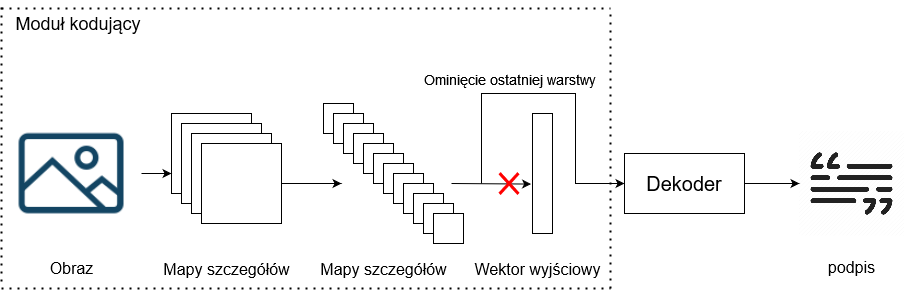
\includegraphics[width=\linewidth]{schemat-pretrained}
    \caption{Diagram przedstawiający architekturę z wykorzystanie wcześniej wyuczonych modeli jako modułów kodujących. Opracowanie własne.}
    \label{fig:schemat-pretrained}
\end{figure}
\noindent Wykorzystane moduły dekodujące:
\begin{itemize}
    \item RNN \cite{rnn} -- podstawowa rekurencyjna sieć neuronowa.
    \item LSTM \cite{lstm} -- jest rozszerzeniem podstawowej rekurencyjnej sieci neuronowej, której głównym celem jest rozwiązanie problemu zanikającego gradientu.
    \item GRU \cite{gru} -- posiada mniej parametrów niż LSTM, co w teorii pozwala na szybsze i wydajniejsze uczenie się.
    \item Transformer \cite{transformer} -- umożliwia na analizowanie pełnej sekwencji w jednym momencie poprzez wykorzystanie modułu atencji.
\end{itemize}
Każda kombinacja modułu kodującego wraz z modułem dekodującym została sprawdzona pod względem:
\begin{itemize}
    \item wydajności uczenia poprzez sprawdzenie czasu potrzebnego na przetworzenie przez architekturę treningowego zbioru danych,
    \item wydajności generowania podpisów, poprzez sprawdzenie czasu potrzebnego na przetworzenie testowego zbioru danych,
    \item efektywności poprzez sprawdzenie skuteczności generowania podpisów.
\end{itemize}
Wydajność testowania oraz skuteczność generowania podpisów została również sprawdzona dla dedykowanej architektury GIT \cite{wang2022git} wykorzystującej transformer wizyjny wraz z klasycznym transformerem. W tym celu wykorzystane zostały wagi udostępnione przez autorów -- pozwoliło to na całkowite pominięcie etapu uczenia tejże sieci.
\subsection{Trenowanie pełnej architektury}
W celu sprawdzenia jak duże znaczenie ma wykorzystanie wstępnie wytrenowanych modułów kodujących, ich wydajność treningowa została porównana do wydajności uczenia pełnej architektury. Porównane zostały wszystkie wcześniej wymienione kombinacje modułów kodujących wraz z modułami dekodującymi. Oprócz tego do zbioru modułów dekodujących dodany został również podstawowy wariant splotowej sieci neuronowej. Moduły zostały połączone w taki sam sposób jak w przypadku wykorzystania wstępnie wytrenowanych wag -- ostatnia warstwa w pełni połączona została usunięta, a dane wyjściowe modułu kodującego są bezpośrednimi danymi wejściowymi modułu dekodującego.
\subsection{Wstępne przetwarzanie danych}
Dane wejściowe w postaci macierzy pikseli obrazów cyfrowych zostały normalizowane, a ich wymiary ujednolicone w celu uproszczenia obliczeń. Natomiast przetwarzanie języka naturalnego odbyło się poprzez zastosowanie tokenizacji -- w tym celu został wykorzystany wcześniej wytrenowany model Distilbert \cite{distilbert}.
\subsection{Metryki}
Oprócz parametrów dotyczących wydajności trenowania oraz testowania podanych rozwiązań sprawdzona została również skuteczność otrzymanych wyników. Wybrane metryki:
\begin{itemize}
    \item BLEU (ang. Bilingual Evaluation Understudy) \cite{bleu} -- metryka oryginalnie wywodząca się z dziedziny tłumaczenia maszynowego, jednakże ze względu na taki sam format danych, idealnie pasuje również do ewaluacji wyników generowania podpisów do obrazów. Zakres wartości metryki zawiera się w przedziale od 0 do 1, gdzie najlepszą wartością jest górna granica. % MAYBE dodać formułe wyliczania oraz informację o n gramach
    \item METEOR (ang. Metric for Evaluation of Translation with Explicit ORdering) \cite{meteor} -- metryka będąca rozwinięciem metryki BLEU. Odznacza się lepszą oceną korelacji na poziomie zdań, a nie tak jak w~przypadku BLEU, na~poziomie całego korpusu. Zakres wartości metryki zawiera się w przedziale od 0 do 1, gdzie najlepszą wartością jest górna granica.
    \item CIDEr (ang. Consensus-based Image Description Evaluation) \cite{cider} -- dedykowana metryka do oceny jakości generowanych opisów obrazów. Poprzez zastosowanie algorytmu TF-IDF \cite{tfidf} pozwala na ocenę jakości generowanych podpisów w oparciu o~podobieństwo do wszystkich podpisów, a nie tylko do jednego. Zakres jej wartości jest większy niż w przypadku pozostałych metryk, ponieważ wynosi od 0 do 10, gdzie wartość 10 oznacza najlepszy wynik.
    \item SPICE -- wykorzystuje ona rozbiór logiczny zdania w celu stworzenie jego grafu, które są następnie porównywane z grafami pozostałych zdań. Dzięki temu metryka ta jest w stanie ocenić podobieństwo poprzez strukturę zdania, a nie tylko występowanie danych słów. Tak jak w przypadku metryk BLEU i METEOR zakres wartości zawiera się w przedziale od 0 do 1, gdzie najlepszą wartością jest górna granica.
\end{itemize}
W przypadku wyników architektur wykorzystujących różne kombinacje modułów kodujących oraz dekodujących zostały one przedstawione poprzez tylko dwie metryki: BLEU i CIDEr. Pozostałe wskaźniki zostały wykorzystane jedynie w przypadku porównania wyników bezpośrednio z wartościami otrzymanymi przez autorów dla dedykowanych rozwiązań. Ograniczenie zostało wprowadzone, w celu zachowania przejrzystości wyników, a także ze względu na fakt, iż metryki BLEU i CIDEr powinny być w pełni wystarczające, aby ocenić jakość generowanych podpisów.
\subsection{Wykorzystane środowiska}
W celu porównania wpływu użytych jednostek obliczeniowych na efektywność badanych architektury wykorzystane zostały różne karty graficzne:
\begin{itemize}
    \item NVIDIA GeForce GTX 1650 4GB -- jednostka GPU,
    \item NVIDIA Tesla T4 16 GB -- jednostka GPU,
    \item Intel Core i7-1280P -- jednostka CPU.
\end{itemize}
W przypadku karty graficznej Tesla T4 wszelkie testy zostały wykonane za pośrednictwem platformy Google Colab umożliwiającej bezpłatny dostęp do zaawansowanych jednostek obliczeniowych. Pozostałe testy zostały wykonane na komputerze osobistym

Docelowa architektura została zaimplementowana przy użyciu gotowych modeli sieci neuronowych zawartych w bibliotekach PyTorch \cite{pytorch} oraz Transformers \cite{wolf-etal-2020-transformers} dostępnych w języku programowania Python.
\subsection{Zbiory danych}
Istnieje wiele zbiorów danych zawierających obrazy wraz z ich opisami. Jednymi z najpopularniejszych są:
\begin{itemize}
    \item MS COCO \cite{mscoco} -- składa się on z ponad 120 tysięcy zdjęć.
    \item Flickr \cite{flickr30k} -- posiada on mniej zdjęć niż zbiór MS COCO, ponieważ jego szeroki wariant zawiera ich 30 tysięcy, natomiast węższy 8 tysięcy.
\end{itemize}
Ze względu na konieczność wytrenowania dużej liczby architektur niezwykle istotne jest dokonanie tego w sensownym oknie czasowym, co może być niewykonalne przy wykorzystaniu zbioru MS COCO. Z tego względu został wykorzystany węższy wariant zbioru Flickr zawierający 8 tysięcy zdjęć. Ten wybór pozwolił również sprawdzić skuteczność modelu GIT bez wcześniejszego go wytrenowania, posługując się jedynie modelem udostępnionym przez autorów, który został wytrenowany na zbiorze MS COCO.
Zbiór danych został podzielony na:
\begin{itemize}
    \item zbiór treningowy -- 6 tysięcy zdjęć,
    \item zbiór testowy -- 1 tysiąc zdjęć,
    \item zbiór walidacyjny -- 1 tysiąc zdjęć.
\end{itemize}

\noindent Wszystkie kombinacje wykorzystanych architektur zostały wyuczone przy pomocy treningowego zbioru danych. Dodatkowo w trakcie treningu jakość modelu była sprawdzana przy pomocy zbioru walidacyjnego. Dane były przetwarzane w seriach liczących po 32 elementy. Przetwarzanie było powtarzane 500 razy.

\newpage % Rozdziały zaczynamy od nowej strony.

\section{Opis przeprowadzonych eksperymentów}
W celu generowania podpisów do obrazków wykorzystana została architektura składającą się z modułu kodującego oraz modułu dekodującego. W eksperymentach zostały wykorzystane ich różne konfiguracje. Dodatkowo wyniki zostały porównane z architekturami dedykowanymi do zadania generowania podpisów.
\subsection{Wykorzystanie wstępnie wytrenowanych modeli}
Szeroką popularnością w dziedzinie trenowania modeli sieci neuronowych cieszy się technika przenoszenia wiedzy. Jest to technika uczenia maszynowego, w której model uczony jest na jednym zadaniu, a następnie wykorzystuje tę wiedzę do lepszego rozwiązania innego, zazwyczaj podobnego zadania. Może zostać ona podzielona na dwa kluczowe kroki:
\begin{itemize}
    \item Początkowe uczenie modelu na dużym zbiorze danych i zadaniu, na którym jest dostępna duża ilość informacji.
    \item  Dostosowanie modelu do nowego zadania. Parametry modelu są dostosowywane do specyfiki nowego zadania, a wagi nauczone podczas początkowe uczenia są używane jako punkt wyjścia.
\end{itemize}
W przypadku generowania podpisów do obrazków technikę przenoszenia wiedzy można zastosować poprzez wykorzystanie wcześniej wyuczonych modeli sieci splotowych w ramach modułu kodującego. Trenowanie splotowych sieci neuronowych od zera na dużym zbiorze danych może być czasochłonne i wymagać dużej ilości zasobów obliczeniowych. Wykorzystanie wstępnie wytrenowanych modeli pozwala uniknąć tego procesu, ponieważ modele te są już przeszkolone do ekstrakcji cech, co jest ich głównym zadaniem w całej architekturze. Z tego względu dane treningowe zostały poddane wcześniejszemu przetworzeniu przez moduł kodujący, a trening polegał na uczeniu jedynie modułu dekodującego. Wykorzystane moduły kodujące:
\begin{itemize}
    \item AlexNet \cite{alexnet} -- jedna z najbardziej wpływowych sieci w historii przetwarzania obrazów, cechuje ją duża liczba parametrów, co pozwala na wyodrębnienie dużej liczby cech.
    \item GoogLeNet \cite{googlenet} -- sieć charakteryzuje się modułami inception mającymi na celu efektywne wykorzystanie zasobów obliczeniowych.
    \item VGGNet \cite{vggnet} -- bardzo głęboka sieć neuronowa wykorzystująca małe filtry splotowe pozwalających na wyodrębnienie cech o różnym stopniu skomplikowania.
    \item ResNet \cite{resnet} -- bardzo głęboka sieć neuronowa charakteryzująca się blokami rezydualnymi, które umożliwiają efektywne uczenie się sieci neuronowej o dużej liczbie warstw.
    \item VIT \cite{vit} - transformer wizyjny będący rozszerzeniem modelu transformer. Implementuje on mechanizm atencji, w celu wyodrębniania poszczególnych cech obrazu.
\end{itemize}
Ze względu na wykorzystanie wstępnie wytrenowanych wag modułów zostały one poddane modyfikacji -- ostatnia warstwa w pełni połączona została usunięta, co zostało przedstawione na rysunku \ref{fig:schemat-pretrained}. Poprzez taką zmianę danymi wyjściowymi tychże sieci są tak zwane mapy szczegółów zawierające wyodrębnione cechy obrazu, które są bezpośrednimi danymi wejściowymi modułu dekodującego.
\begin{figure}[H]
    \centering
    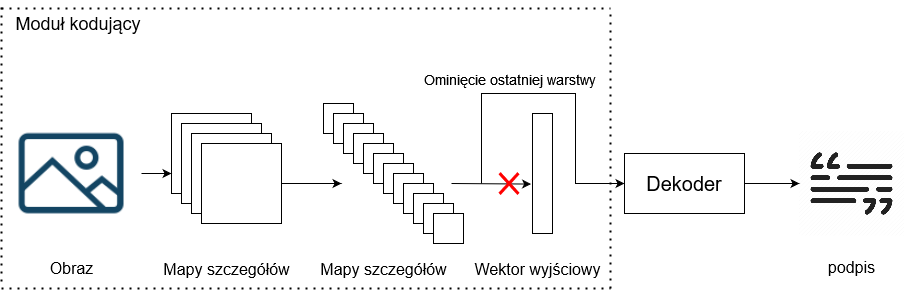
\includegraphics[width=\linewidth]{schemat-pretrained}
    \caption{Diagram przedstawiający architekturę z wykorzystanie wcześniej wyuczonych modeli jako modułów kodujących. Opracowanie własne.}
    \label{fig:schemat-pretrained}
\end{figure}
\noindent Wykorzystane moduły dekodujące:
\begin{itemize}
    \item RNN \cite{rnn} -- podstawowa rekurencyjna sieć neuronowa.
    \item LSTM \cite{lstm} -- jest rozszerzeniem podstawowej rekurencyjnej sieci neuronowej, której głównym celem jest rozwiązanie problemu zanikającego gradientu.
    \item GRU \cite{gru} -- posiada mniej parametrów niż LSTM, co w teorii pozwala na szybsze i wydajniejsze uczenie się.
    \item Transformer \cite{transformer} -- umożliwia na analizowanie pełnej sekwencji w jednym momencie poprzez wykorzystanie modułu atencji.
\end{itemize}
Każda kombinacja modułu kodującego wraz z modułem dekodującym została sprawdzona pod względem:
\begin{itemize}
    \item wydajności uczenia poprzez sprawdzenie czasu potrzebnego na przetworzenie przez architekturę treningowego zbioru danych,
    \item wydajności generowania podpisów, poprzez sprawdzenie czasu potrzebnego na przetworzenie testowego zbioru danych,
    \item efektywności poprzez sprawdzenie skuteczności generowania podpisów.
\end{itemize}
Wydajność testowania oraz skuteczność generowania podpisów została również sprawdzona dla dedykowanej architektury GIT \cite{wang2022git} wykorzystującej transformer wizyjny wraz z klasycznym transformerem. W tym celu wykorzystane zostały wagi udostępnione przez autorów -- pozwoliło to na całkowite pominięcie etapu uczenia tejże sieci.
\subsection{Trenowanie pełnej architektury}
W celu sprawdzenia jak duże znaczenie ma wykorzystanie wstępnie wytrenowanych modułów kodujących, ich wydajność treningowa została porównana do wydajności uczenia pełnej architektury. Porównane zostały wszystkie wcześniej wymienione kombinacje modułów kodujących wraz z modułami dekodującymi. Oprócz tego do zbioru modułów dekodujących dodany został również podstawowy wariant splotowej sieci neuronowej. Moduły zostały połączone w taki sam sposób jak w przypadku wykorzystania wstępnie wytrenowanych wag -- ostatnia warstwa w pełni połączona została usunięta, a dane wyjściowe modułu kodującego są bezpośrednimi danymi wejściowymi modułu dekodującego.
\subsection{Wstępne przetwarzanie danych}
Dane wejściowe w postaci macierzy pikseli obrazów cyfrowych zostały normalizowane, a ich wymiary ujednolicone w celu uproszczenia obliczeń. Natomiast przetwarzanie języka naturalnego odbyło się poprzez zastosowanie tokenizacji -- w tym celu został wykorzystany wcześniej wytrenowany model Distilbert \cite{distilbert}.
\subsection{Metryki}
Oprócz parametrów dotyczących wydajności trenowania oraz testowania podanych rozwiązań sprawdzona została również skuteczność otrzymanych wyników. Wybrane metryki:
\begin{itemize}
    \item BLEU (ang. Bilingual Evaluation Understudy) \cite{bleu} -- metryka oryginalnie wywodząca się z dziedziny tłumaczenia maszynowego, jednakże ze względu na taki sam format danych, idealnie pasuje również do ewaluacji wyników generowania podpisów do obrazów. Zakres wartości metryki zawiera się w przedziale od 0 do 1, gdzie najlepszą wartością jest górna granica. % MAYBE dodać formułe wyliczania oraz informację o n gramach
    \item METEOR (ang. Metric for Evaluation of Translation with Explicit ORdering) \cite{meteor} -- metryka będąca rozwinięciem metryki BLEU. Odznacza się lepszą oceną korelacji na poziomie zdań, a nie tak jak w~przypadku BLEU, na~poziomie całego korpusu. Zakres wartości metryki zawiera się w przedziale od 0 do 1, gdzie najlepszą wartością jest górna granica.
    \item CIDEr (ang. Consensus-based Image Description Evaluation) \cite{cider} -- dedykowana metryka do oceny jakości generowanych opisów obrazów. Poprzez zastosowanie algorytmu TF-IDF \cite{tfidf} pozwala na ocenę jakości generowanych podpisów w oparciu o~podobieństwo do wszystkich podpisów, a nie tylko do jednego. Zakres jej wartości jest większy niż w przypadku pozostałych metryk, ponieważ wynosi od 0 do 10, gdzie wartość 10 oznacza najlepszy wynik.
    \item SPICE -- wykorzystuje ona rozbiór logiczny zdania w celu stworzenie jego grafu, które są następnie porównywane z grafami pozostałych zdań. Dzięki temu metryka ta jest w stanie ocenić podobieństwo poprzez strukturę zdania, a nie tylko występowanie danych słów. Tak jak w przypadku metryk BLEU i METEOR zakres wartości zawiera się w przedziale od 0 do 1, gdzie najlepszą wartością jest górna granica.
\end{itemize}
W przypadku wyników architektur wykorzystujących różne kombinacje modułów kodujących oraz dekodujących zostały one przedstawione poprzez tylko dwie metryki: BLEU i CIDEr. Pozostałe wskaźniki zostały wykorzystane jedynie w przypadku porównania wyników bezpośrednio z wartościami otrzymanymi przez autorów dla dedykowanych rozwiązań. Ograniczenie zostało wprowadzone, w celu zachowania przejrzystości wyników, a także ze względu na fakt, iż metryki BLEU i CIDEr powinny być w pełni wystarczające, aby ocenić jakość generowanych podpisów.
\subsection{Wykorzystane środowiska}
W celu porównania wpływu użytych jednostek obliczeniowych na efektywność badanych architektury wykorzystane zostały różne karty graficzne:
\begin{itemize}
    \item NVIDIA GeForce GTX 1650 4GB -- jednostka GPU,
    \item NVIDIA Tesla T4 16 GB -- jednostka GPU,
    \item Intel Core i7-1280P -- jednostka CPU.
\end{itemize}
W przypadku karty graficznej Tesla T4 wszelkie testy zostały wykonane za pośrednictwem platformy Google Colab umożliwiającej bezpłatny dostęp do zaawansowanych jednostek obliczeniowych. Pozostałe testy zostały wykonane na komputerze osobistym

Docelowa architektura została zaimplementowana przy użyciu gotowych modeli sieci neuronowych zawartych w bibliotekach PyTorch \cite{pytorch} oraz Transformers \cite{wolf-etal-2020-transformers} dostępnych w języku programowania Python.
\subsection{Zbiory danych}
Istnieje wiele zbiorów danych zawierających obrazy wraz z ich opisami. Jednymi z najpopularniejszych są:
\begin{itemize}
    \item MS COCO \cite{mscoco} -- składa się on z ponad 120 tysięcy zdjęć.
    \item Flickr \cite{flickr30k} -- posiada on mniej zdjęć niż zbiór MS COCO, ponieważ jego szeroki wariant zawiera ich 30 tysięcy, natomiast węższy 8 tysięcy.
\end{itemize}
Ze względu na konieczność wytrenowania dużej liczby architektur niezwykle istotne jest dokonanie tego w sensownym oknie czasowym, co może być niewykonalne przy wykorzystaniu zbioru MS COCO. Z tego względu został wykorzystany węższy wariant zbioru Flickr zawierający 8 tysięcy zdjęć. Ten wybór pozwolił również sprawdzić skuteczność modelu GIT bez wcześniejszego go wytrenowania, posługując się jedynie modelem udostępnionym przez autorów, który został wytrenowany na zbiorze MS COCO.
Zbiór danych został podzielony na:
\begin{itemize}
    \item zbiór treningowy -- 6 tysięcy zdjęć,
    \item zbiór testowy -- 1 tysiąc zdjęć,
    \item zbiór walidacyjny -- 1 tysiąc zdjęć.
\end{itemize}

\noindent Wszystkie kombinacje wykorzystanych architektur zostały wyuczone przy pomocy treningowego zbioru danych. Dodatkowo w trakcie treningu jakość modelu była sprawdzana przy pomocy zbioru walidacyjnego. Dane były przetwarzane w seriach liczących po 32 elementy. Przetwarzanie było powtarzane 500 razy.

\newpage % Rozdziały zaczynamy od nowej strony.

\section{Wyniki}
Poniższe dane przedstawione na rysunku \ref{fig:memories} prezentują ilość pamięci RAM wyrażonej w gigabajtach potrzebnej do uruchomienia poszczególnych architektur dla rozwiązania klasycznego oraz wykorzystującego wektor składający się z danych z map szczegółów sieci splotowych.
\begin{figure}[H]
    \centering
    \begin{subfigure}{.5\textwidth}
        \centering
        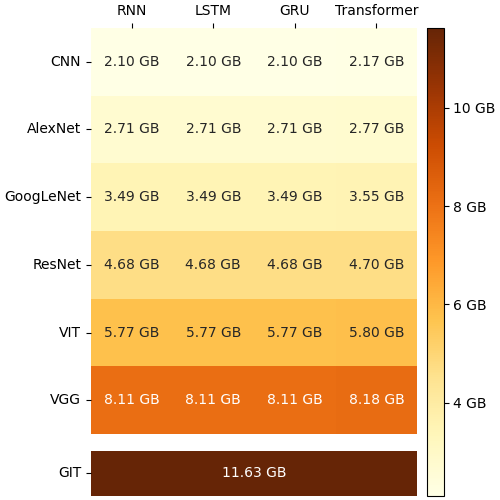
\includegraphics[width=.99\linewidth]{timings/ram}
        \caption{Klasyczne połączenie.}
        \label{fig:memory}
    \end{subfigure}%
    \centering
    \begin{subfigure}{.5\textwidth}
        \centering
        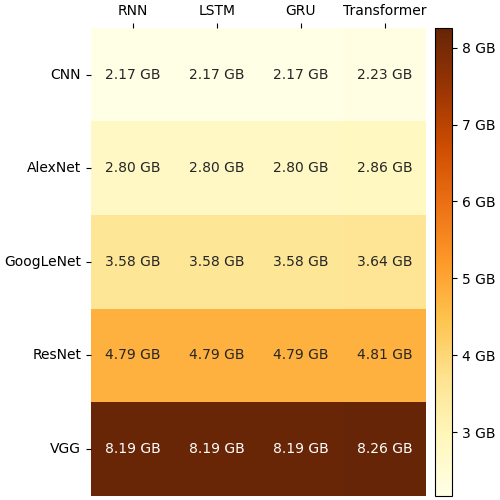
\includegraphics[width=.99\linewidth]{timings/ram_modified}
        \caption{Połączenie wykorzystujące mapy szczegółów.}
        \label{fig:memory-modified}
    \end{subfigure}%
    \caption{Pamięć RAM potrzebna do uruchomienia testowanych architektur wyrażona w gigabajtach. Opracowanie własne.}
    \label{fig:memories}
\end{figure}
\noindent Można zauważyć, iż największe różnice w ilości potrzebnej pamięci RAM są pomiędzy poszczególnymi modułami kodującymi. W przypadku modułów dekodujących zauważalna różnica jest pomiędzy wykorzystaniem transformera a pozostałymi sieciami rekurencyjnymi. Najpewniej wynika to z tego, iż sieci rekurencyjne przetwarzają tylko jeden element w danym czasie w przeciwieństwie do transformera, który przy pomocy modułu atencji analizuje całą sekwencję w jednym momencie, przez co konieczne jest jej załadowanie do pamięci komputera. Istotnym jest również fakt, iż połowa modułów kodujących potrzebuje ponad 4 GB pamięci, a co za tym idzie, nie było możliwe ich wykorzystanie przy pomocy karty graficznej Nvidia GeForce GTX 1650, ponieważ posiada ona tylko cztery gigabajty pamięci. Tak duża ilość potrzebnej pamięci dotyczy bardzo głębokich sieci oraz wykorzystujących transformer wizyjny. Powodem takiego stanu rzeczy jest fakt, iż w przypadku bardzo głębokich sieci splotowych architektura posiada ogromną liczbę parametrów ze względu na dużą liczbę małych filtrów oraz warstw. Natomiast transformer wizyjny przetwarza obraz do postaci sekwencji, która musi być załadowana w całości, co również znacząco wpływa na rozmiar potrzebnej pamięci. Warto również zauważyć, iż wykorzystanie danych pochodzących z map szczegółów sieci splotowych, tylko nieznacznie wpłynęło na zwiększenie wykorzystywanej pamięci RAM. Wpływ tutaj miało wykorzystanie warstw w pełni połączonych, które w porównaniu do warstw splotowych nie są aż tak obciążające i zajmują stosunkowo mniejszą ilość pamięci.

\subsection{Wydajność uczenia modułów dekodujących dla połączenia klasycznego}
Dane przedstawione na rysunku \ref{fig:timings-decoders} prezentują czas potrzebny na przetworzenie jednej epoki treningowej poszczególnych kombinacji modułów kodujących oraz dekodujących wykorzystujących wcześniej wytrenowane moduły kodujące przy pomocy klasycznego połączenia.
\begin{figure}[H]
    \centering
    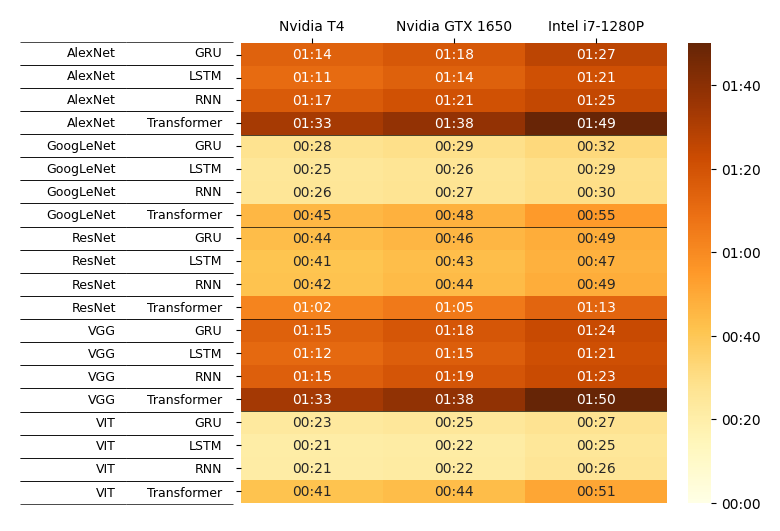
\includegraphics[width=.9\linewidth]{timings/timings_decoders}
    \caption{Czas potrzebny na przetworzenie jednej epoki treningowej poszczególnych kombinacji modułów kodujących oraz dekodujących wykorzystujących wcześniej wytrenowane moduły kodujące. Dane przedstawione w skali logarytmicznej. Opracowanie własne.}
    \label{fig:timings-decoders}
\end{figure}
\noindent Ponownie tak jak w przypadku potrzebnej pamięci do alokacji architektury tutaj również najbardziej zauważalne są różnice czasowe pomiędzy poszczególnymi modułami kodującymi. W przypadku modułów dekodujących różnice są widoczne jedynie pomiędzy wykorzystaniem transformera a pozostałymi sieciami rekurencyjnymi. Co ciekawe, długość przetwarzania nie jest zależna od stopnia skomplikowania sieci. Ze względu na wcześniejsze wygenerowanie danych wejściowych do modułów dekodujących poprzez przetworzenie obrazów przy pomocy wstępnie wyuczonych modułów kodujących, czas potrzebny na przetworzenie jednej epoki treningowej jest zależny od wielkości ostatniej warstwy modułu kodującego, który jest następujący dla poszczególnych sieci:
\begin{itemize}
    \item AlexNet -- 4096,
    \item GoogLeNet -- 1024,
    \item VGGNet -- 4096,
    \item ResNet -- 2048,
    \item VIT -- 768.
\end{itemize}
Biorąc to pod uwagę, łatwo można zauważyć, iż sieć z najmniejszą warstwą końcową, czyli VIT, potrzebuje najmniej czasu na przetworzenie jednej epoki treningowej, a sieci z największą warstwą końcową, czyli AlexNet oraz VGGNet, potrzebuje go najwięcej. W przypadku trenowania również modułu kodującego bez zastosowania wstępnie wyuczonych modeli możliwe byłoby dostosowanie wielkości ostatniej warstwy, w celu zmniejszenia czasu potrzebnego na przetworzenie danych przez moduł dekodujący.
\subsection{Wydajność uczenia architektury dla zaproponowanego połączenia}
W przypadku wykorzystania dodatkowych danych pochodzących z pośrednich warstw splotowych konieczne było zastosowanie warstw w pełni połączonych, które również musiały zostać wytrenowane wraz z modułem dekodującym. Dane przedstawione na rysunku \ref{fig:timings-decoders-modified} prezentują czas potrzebny na przetworzenie jednej epoki treningowej poszczególnych kombinacji modułów kodujących oraz dekodujących wykorzystujących wcześniej wytrenowane moduły kodujące przy pomocy zaproponowanego połączenia.
\begin{figure}[H]
    \centering
    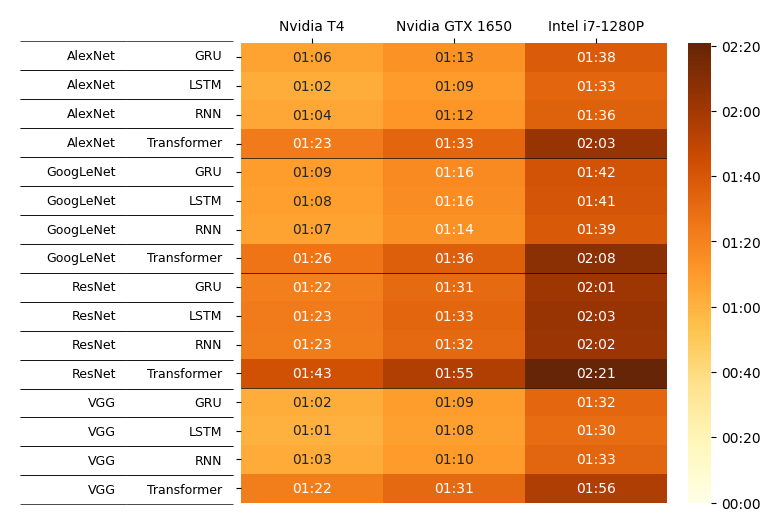
\includegraphics[width=.9\linewidth]{timings/timings_decoders_modified}
    \caption{Czas potrzebny na przetworzenie jednej epoki treningowej poszczególnych kombinacji modułów kodujących oraz dekodujących wykorzystujących wcześniej wytrenowane moduły kodujące przy pomocy zaproponowanego połączenia. Opracowanie własne.}
    \label{fig:timings-decoders-modified}
\end{figure}
\noindent Ze względu na generowanie wektorów wejściowych o takich samych rozmiarach dla każdego z modułów kodujących, różnica pomiędzy ich poszczególnymi typami nie jest tak widoczna, jak w przypadku klasycznego podejścia. W przypadku sieci AlexNet oraz VGG, których rozmiar wyjściowych wektorów pozostał niezmienny, wzrost czasu jest na poziomie około 10\%, co jest przewidywalną różnicą ze względu na konieczność wyuczenia również warstw w pełni połączonych odpowiedzialnych za redukcję rozmiaru wektorów pochodzących z warstw splotowych. Tak jak w poprzednim przypadku, ponownie można zauważyć różnicę pomiędzy sieciami rekurencyjnymi a transformerem. Również warto zwrócić uwagę na to, iż wykorzystanie jednostki GPU miało pewien wpływ na wydajność treningu, ale nie była to drastyczna poprawa -- w większości przypadków spadek czasu wyniósł około 25\% w przypadku podstawowej jednostki GPU, a około 30\% w przypadku jednostki specjalistycznej w porównaniu do jednostki CPU. Można stwierdzić, iż wykorzystanie danych z warstw splotowych miało wpływ na długość treningu, mimo iż jest to jedynie kilka sekund przetwarzania epoki, biorąc pod uwagę fakt, iż w przypadku trenowania sieci konieczne jest przetworzenie danych kilkaset razy, różnica ta staje się znacząca -- przetworzenie 250 epok daje różnicę na poziomie 45 minut.
\subsection{Wydajność uczenia modułów kodujących oraz dekodujących}
Dane przedstawione na rysunku \ref{fig:timings-networks} prezentują czas potrzebny na przetworzenie jednej epoki treningowej poszczególnych kombinacji modułów kodujących oraz dekodujących.
\begin{figure}[H]
    \centering
    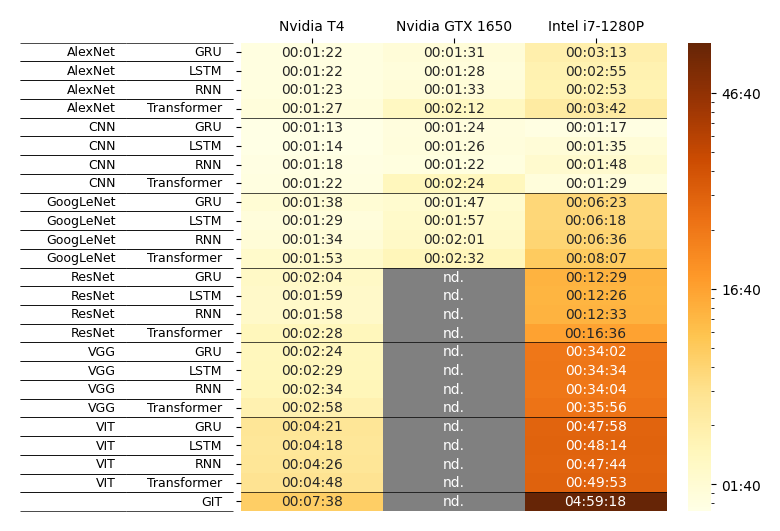
\includegraphics[width=.9\linewidth]{timings/timings_networks}
    \caption{Czas potrzebny na przetworzenie jednej epoki treningowej poszczególnych kombinacji modułów kodujących oraz dekodujących. Opracowanie własne.}
    \label{fig:timings-networks}
\end{figure}
\noindent Niestety ze względu na ograniczenie pamięci RAM karty graficznej Nvidia GTX 1650 nie było możliwe przeprowadzenie treningu sieci zajmujących więcej niż 4 GB pamięci, czyli ResNet, VGG, VIT oraz GIT. W przypadku czasu potrzebnego na przetworzenie danych przy pomocy jednostki CPU rośnie on w sposób wykładniczy. Biorąc pod uwagę, iż założeniem przeprowadzonych eksperymentów było przetworzenie zbioru treningowej 500 razy, dla połowy sieci staje się to niewykonalne. Już w przypadku sieci GoogleNet połączonej z jedną z sieci rekurencyjnych, gdzie jedna epoka treningowa zajmuje ponad 6 minut, powtórzenie jej 500 razy zajęłoby 53 godziny. Natomiast w przypadku najdłużej przetwarzającej sieci, czyli GIT, czas ten wyniósłby ponad 100 dni ciągłego przetwarzania. W przypadku pozostałych sieci, gdzie czas kilkudziesięciu godzin jest w wielu momentach akceptowalnym rzędem wielkości, to tak wydłużony czas uczenia znacząco utrudnia reagowanie na wszelkie błędy oraz problemy. Sytuacja jest znacznie lepsza w przypadku wykorzystania jednostki GPU. Pomiędzy modelem dostępnym w wielu komputerach stacjonarnych, Nvidia GTX 1650, a modelem dedykowanym do obliczeń na kartach graficznych, Nvidia T4, różnice są stosunkowo niewielkie. W przypadku architektury GIT przetworzenie danych 500 razy zajęłoby około 65 godzin, co w porównaniu do czasu potrzebnego w przypadku wykorzystania jednostki CPU jest osiągalne. Dodatkowo warto wspomnieć, iż korelacja pomiędzy liczbą parametrów ostatniej warstwy modułu kodującego a czasem potrzebny na trening nie pojawia się w tym przypadku. Wynika to z faktu, iż czas trenowania modułu kodującego rośnie o wiele znaczniej wraz z większym skomplikowaniem wykorzystanej architektury. Z tego względu również różnice pomiędzy architekturami wykorzystującymi klasyczne połączenie modułów a tymi wykorzystującymi dodatkowe dane z warstw splotowych nie są aż tak zauważalne -- wzrost czasu treningu jest nieznaczny w porównaniu do całościowego czasu przetwarzania, co można zauważyć na rysunku \ref{fig:timings-networks-modified}.
\begin{figure}[H]
    \centering
    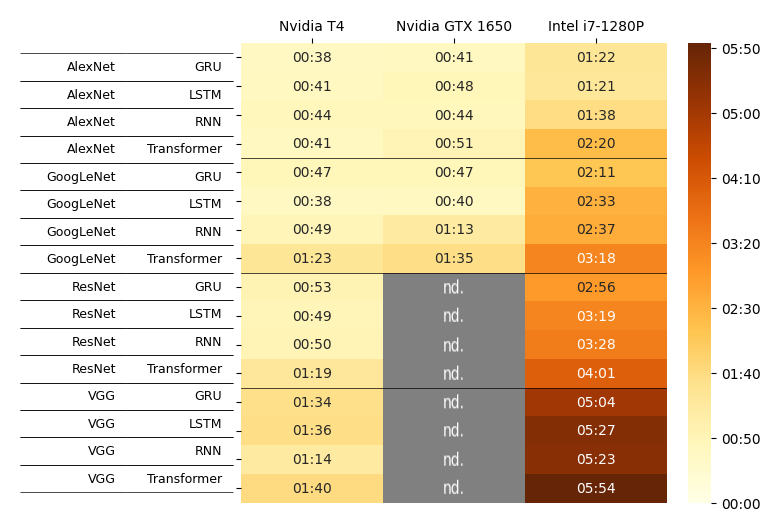
\includegraphics[width=.9\linewidth]{timings/timings_inference_decoders_modified}
    \caption{Czas potrzebny na przetworzenie jednej epoki treningowej poszczególnych kombinacji modułów kodujących oraz dekodujących wykorzystujących dane z warstw splotowych. Opracowanie własne.}
    \label{fig:timings-networks-modified}
\end{figure}
\noindent Różnica w czasie trenowania pomiędzy klasyczną techniką połączenia modułu kodującego i dekodującego a zaproponowanym rozwiązaniem wykorzystującym dane z warstw splotowych jest bardzo zbliżona w obu przypadkach -- trenowania modułu dekodującego oraz całej architektury. Jest to przewidywalny rezultat, ponieważ w obu podejściach dodatkowe obciążenie jest takie samo -- konieczność wyuczenia dodatkowych warstw w pełni połączonych.
\subsection{Wydajność generowania podpisów}
Na rysunku \ref{fig:timings-decoders-inference} zostały przedstawione czasy potrzebne na wygenerowanie podpisów obrazków pochodzących z testowego zbioru danych dla poszczególnych architektur.
\begin{figure}[H]
    \centering
    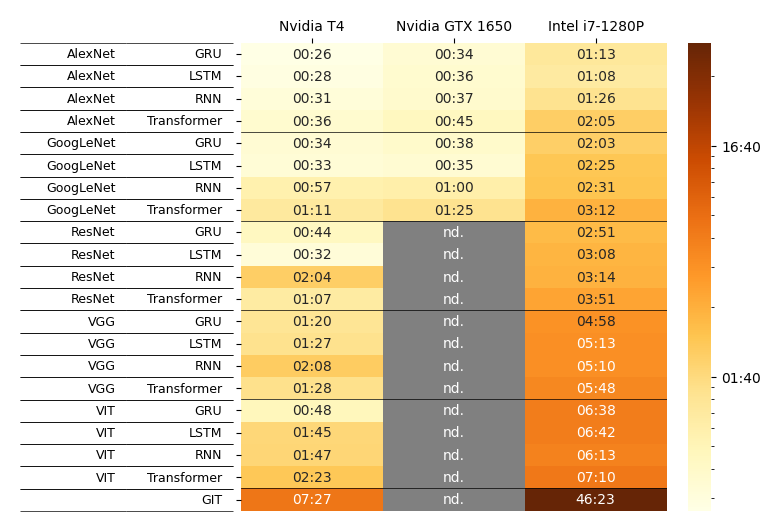
\includegraphics[width=.9\linewidth]{timings/timings_inference_decoders}
    \caption{Czas potrzebny na wygenerowanie podpisów obrazków pochodzących z testowego zbioru danych dla poszczególnych architektur, które zostały wyuczone przy użyciu wcześniej wytrenowanych modułów kodujących, wykorzystując klasyczne połączenie modułów. Dane przedstawione w skali logarytmicznej. Opracowanie własne.}
    \label{fig:timings-decoders-inference}
\end{figure}
\noindent W przypadku generowania podpisów konieczne jest wykorzystanie bezpośrednio modułu kodującego, ponieważ w warunkach naturalnych przetwarzane zdjęcie nie jest wcześniej znane. Z tego względu wyniki dla modeli wykorzystujących wcześniej wyuczone moduły kodujące oraz modele trenowane od zera są takie same -- w obu przypadkach obraz przetwarzany jest w ten sam sposób. Wskutek tego nie było możliwe przeprowadzenie eksperymentów przy użyciu karty graficznej Nvidia GTX 1650, tych sieci, których alokacja przekracza 4 GB pamięci. Czas wymagany do przetworzenia zbioru testowego, tak jak w przypadku uczenia architektur, wraz z wykorzystaniem bardziej rozbudowanego modułu kodującego wzrasta, a w przypadku modułów dekodujących znaczące różnice są widoczne jedynie pomiędzy transformerem a pozostałymi sieciami. Ponownie najbardziej wymagającą architekturą okazało się rozwiązanie GIT. Przy jego pomocy przetworzenie tysiąca zdjęć zajęłoby ponad 45 minut, co daje niecałe 3 sekundy na zdjęcie -- taki czas w wielu przypadkach można uznać za akceptowalny, jednakże ponownie pokazuje to, iż prostsze sieci są bardziej przystępne dla osób z ograniczonymi zasobami sprzętowymi. Najszybsza okazała się sieć AlexNet połączona z siecią GRU -- w tym przypadku przetworzenie całego zbioru testowego zajmuje mniej niż pół minuty.
W przypadku wykorzystania danych z wewnętrznych warstw splotowych modułu kodującego, w celu wygenerowania wektora wejściowego modułu kodującego czas generowania podpisów nie zmienił się znacząco, co można zauważyć na rysunku \ref{fig:timings-decoders-inference-modified}.
\begin{figure}[H]
    \centering
    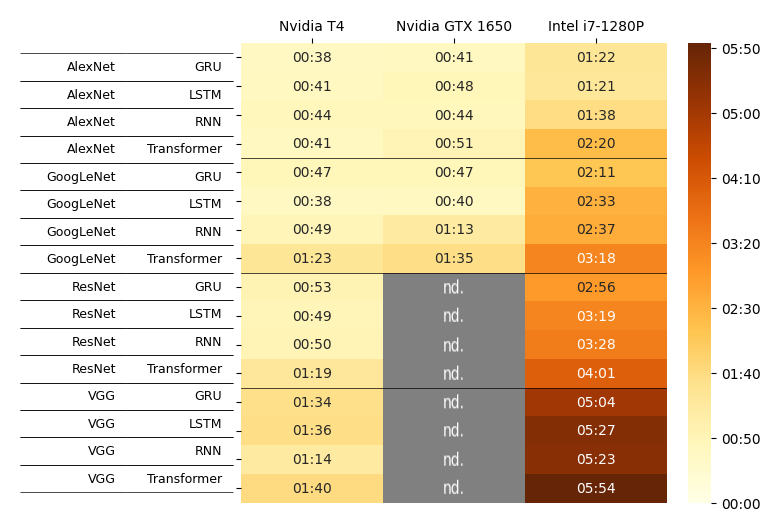
\includegraphics[width=.9\linewidth]{timings/timings_inference_decoders_modified}
    \caption{Czas potrzebny na wygenerowanie podpisów obrazków pochodzących z testowego zbioru danych dla poszczególnych architektur, które zostały wyuczone przy użyciu wcześniej wytrenowanych modułów kodujących, wykorzystując dane z warstw splotowych. Dane przedstawione w skali logarytmicznej. Opracowanie własne.}
    \label{fig:timings-decoders-inference-modified}
\end{figure}
\noindent Tak jak w pozostałych przypadkach, główna różnica czasowa pomiędzy klasycznym podejściem a wykorzystaniem warstw splotowych wynika z konieczności przetworzenia danych przy pomocy dodatkowych warstw w pełni połączonych. Wzrost czasu wynosi kilka sekund i nie jest to znacząco różnica, biorąc pod uwagę długość przetwarzania całego zbioru testowego.
\subsection{Skuteczność architektury wykorzystującej klasyczne połączenie}
Wydajność architektur jest niezwykle istotna, ale by móc w pełni ocenić ich przydatność, konieczne jest sprawdzenie skuteczności generowania podpisów. W tym celu wykorzystane zostały metryki BLEU oraz CIDEr. Dane przedstawione na rysunku \ref{fig:metrics} prezentują wartości tychże metryk dla architektury GIT oraz poszczególnych kombinacji modułów kodujących i dekodujących. Wyraźnie widoczna jest bardzo duża skuteczność architektury GIT. W przypadku metryki BLEU jest ona większa jedynie o 0,02 od drugiej najlepszej architektury -- kodera VIT połączonego z transformerem, ale w przypadku metryki CIDEr różnica ta jest już znacznie większa, ponieważ wynosi aż 0,16. Może to świadczyć o lepszej jakości generowanych podpisach. W przypadku wykorzystywania sieci RNN osiągnięcie sensownych wyników było niemożliwe.
\begin{figure}[H]
    \centering
    \begin{subfigure}{.5\textwidth}
        \centering
        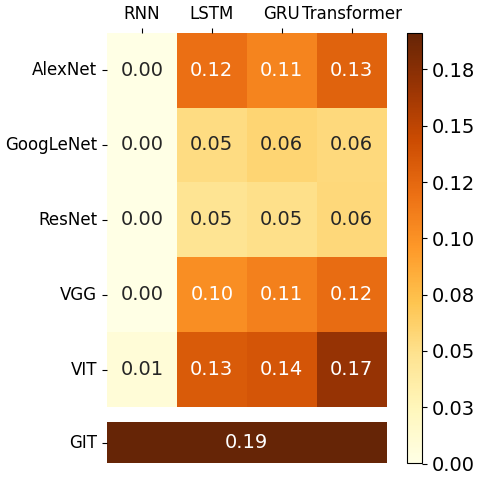
\includegraphics[width=.95\linewidth]{metrics/BLEU}
        \caption{Wartości metryki BLEU}
        \label{fig:bleu}
    \end{subfigure}%
    \centering
    \begin{subfigure}{.5\textwidth}
        \centering
        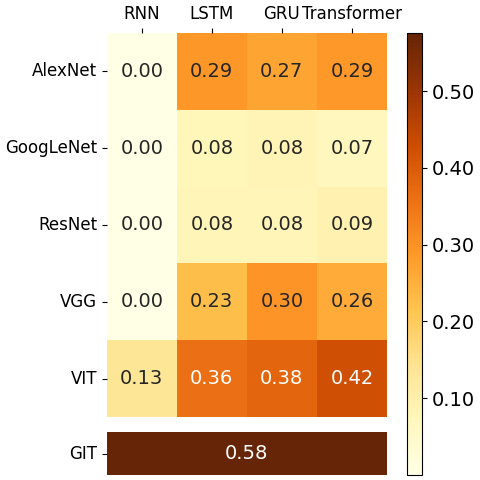
\includegraphics[width=.95\linewidth]{metrics/CIDEr}
        \caption{Wartości metryki CIDEr}
        \label{fig:cider}
    \end{subfigure}%
    \caption{Wartości metryk BLEU oraz CIDEr dla poszczególnych kombinacji modułów kodujących i dekodujących. Opracowanie własne}
    \label{fig:metrics}
\end{figure}
\noindent W prawie wszystkich przypadkach funkcja straty zbioru walidacyjnego szybko osiągała swoje minimum, zaczynała rosnąć, co najczęściej sygnalizuje przeuczenie modelu -- można to zauważyć na rysunku \ref{fig:training-alexnet-rnn}.
\begin{figure}[H]
    \centering
    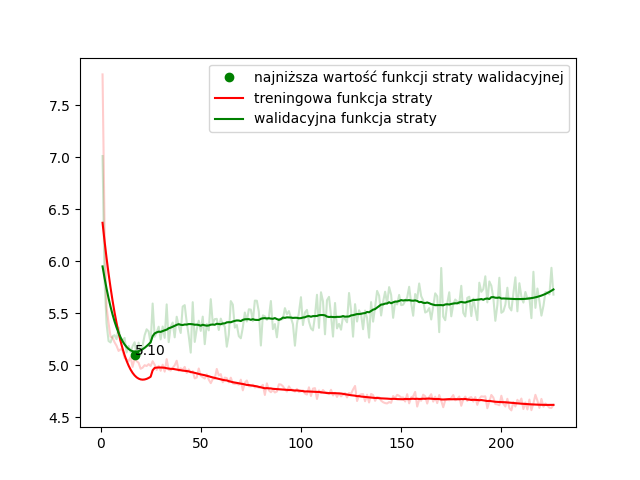
\includegraphics[width=.85\linewidth]{training/alexnet_rnn}
    \caption{Wykres wartości funkcji straty treningowej oraz walidacyjnej dla architektury składającej się z sieci AlexNet i RNN. Opracowanie własne.}
    \label{fig:training-alexnet-rnn}
\end{figure}
\noindent Architektura z wartością funkcji straty na poziomie 5 generowała zdania zawierające jedynie literę „a”, ponieważ jest ona jednym z najczęściej występujących słów w języku angielskim. Wyjątkiem w przypadku wykorzystania sieci RNN jest jej połączenie z transformerem wizyjnym. Dla takiego połączenia metryka BLEU wynosi jedynie 0,01, jednakże wartość CIDEr jest już znacznie wyższa i wynosi 0,13. Wynika to z tego, iż modelowi nie udało się wygenerować pełnych zdań, a jedynie pojedyncze słowa. Przykładowe wyniki zostały przedstawione na rysunku \ref{fig:results-vit-rnn}. Metryka BLEU bierze pod uwagę długość wygenerowanego podpisu, dlatego też w przypadku wygenerowania jedynie pojedynczego słowa, wartość tej metryki jest o wiele niższa w porównaniu do metryki CIDEr.
\begin{figure}[H]
    \centering
    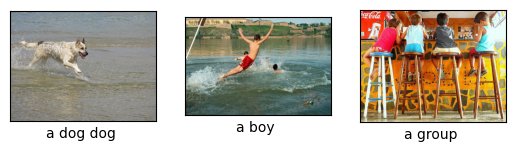
\includegraphics[width=.9\linewidth]{results/vit_rnn}
    \caption{Przykładowe obraz wraz z podpisami wygenerowanymi przez architekturę wykorzystującą transformer wizyjny wraz z siecią RNN. Opracowanie własne.}
    \label{fig:results-vit-rnn}
\end{figure}
\noindent W przypadku tego połączenia funkcja straty walidacyjnej wyniosła wartość 4,5, co można zaobserwować na rysunku \ref{fig:training-vit-rnn}.
\begin{figure}[H]
    \centering
    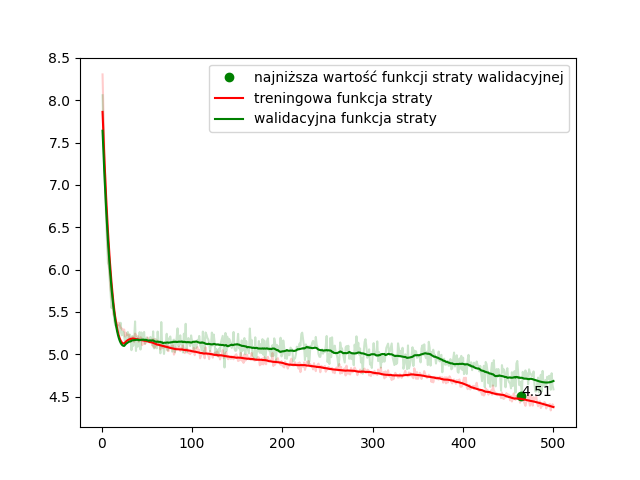
\includegraphics[width=.9\linewidth]{training/vit_rnn}
    \caption{Wykres wartości funkcji straty treningowej oraz walidacyjnej dla architektury składającej się z transformera wizyjnego i sieci RNN. Opracowanie własne.}
    \label{fig:training-vit-rnn}
\end{figure}
\noindent Jest to stosunkowo lepszy wynik od pozostałych architektur zawierających sieć RNN, biorąc również pod uwagę fakt, iż w przeciwieństwie do pozostałych rozwiązań na wykresie funkcji straty widać dalszy potencjał na malenie jej wartości, a co za tym idzie na nawet lepsze wyniki. Niestety ze względu na ograniczenia czasowe narzucony został limit 500 epok treningowych, które architektura łącząca VIT oraz RNN osiągnęła. Jednocześnie warto zauważyć, że wyuczenie modelu zajęło podobny przedział czasowy, co architektura zawierająca sieć GRU oraz LSTM. W obu tych przypadkach średnia potrzebna na przetworzenie jednej epoki treningowej wyniosła mniej niż 30 sekund, co przy 500 epokach treningowych wynosi około 3 godzin, co jest bardzo zadowalającym czasem. Mimo widocznego potencjału sieci RNN w przypadku połączenia z transformerem wizyjnym nie jest to rozwiązanie, które można uznać za satysfakcjonujące, ponieważ w przypadku wykorzystania sieci RNN w połączeniu z innymi modułami kodującymi, nie udało się osiągnąć zadowalających wyników, a w przypadku wykorzystania transformerów wizyjnych, nie jest to rozwiązanie wydajne ze względu na potrzebę wykorzystania takich samych zasobów komputerowych jak w przypadku wykorzystania sieci GRU lub LSTM. Patrząc na krzywą funkcji straty architektury VIT wraz z siecią GRU widoczne na rysunku \ref{fig:training-vit-gru} można zauważyć jej spłaszczenie w ostatnich epokach treningowych, co nie jest widoczne w przypadku wcześniej omawianego połączenia VIT oraz RNN, jak również w przypadku VIT wraz z klasycznym transformerem, co zostało przedstawione na rysunku \ref{fig:training-vit-transformer}.
\begin{figure}[H]
    \centering
    \begin{subfigure}{.5\textwidth}
        \centering
        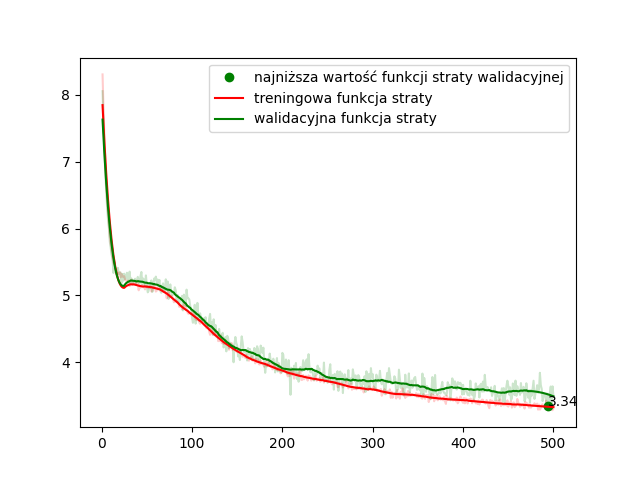
\includegraphics[width=.99\linewidth,trim={1cm 0 1cm 0},clip]{training/vit_gru}
        \caption{GRU}
        \label{fig:training-vit-gru}
    \end{subfigure}%
    \centering
    \begin{subfigure}{.5\textwidth}
        \centering
        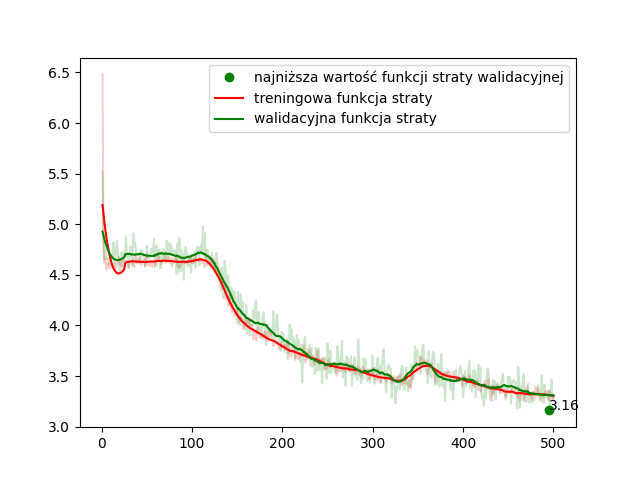
\includegraphics[width=.99\linewidth,trim={1cm 0 1cm 0},clip]{training/vit_transformer_v2}
        \caption{Transformer}
        \label{fig:training-vit-transformer}
    \end{subfigure}%
    \caption{Wykres wartości funkcji straty treningowej oraz walidacyjnej dla architektury składającej się z transformera wizyjnego wraz z różnymi modułami dekodującymi. Opracowanie własne.}
    \label{fig:training-vit-gru-transformer}
\end{figure}
% \begin{figure}[H]
%     \centering
%     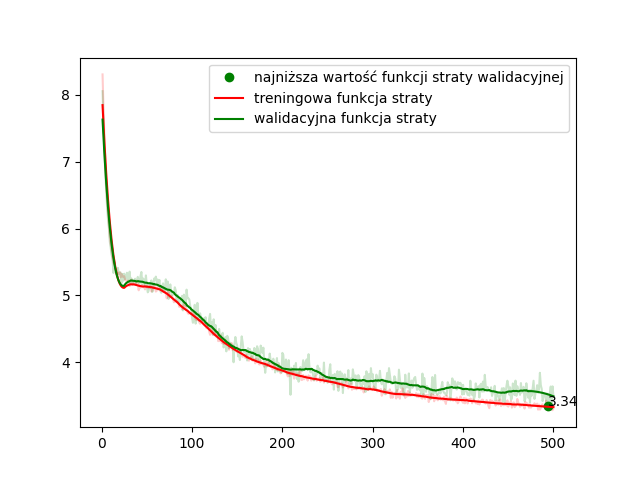
\includegraphics[width=.9\linewidth]{training/vit_gru}
%     \caption{Wykres wartości funkcji straty treningowej oraz walidacyjnej dla architektury składającej się z transformera wizyjnego i sieci GRU. Opracowanie własne.}
%     \label{fig:training-vit-gru}
% \end{figure}
% \begin{figure}[H]
%     \centering
%     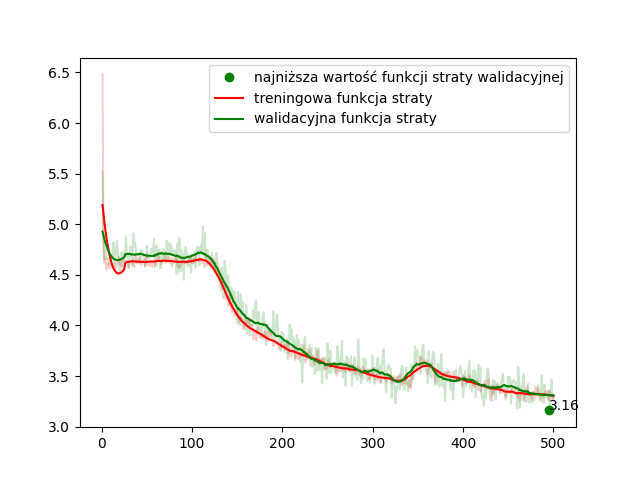
\includegraphics[width=.9\linewidth]{training/vit_transformer_v2}
%     \caption{Wykres wartości funkcji straty treningowej oraz walidacyjnej dla architektury składającej się z transformera wizyjnego i klasycznego. Opracowanie własne.}
%     \label{fig:training-vit-transformer}
% \end{figure}
\noindent Przypadek architektury zawierającej transformer wizyjny i klasyczny jest o wiele bardziej obiecujący niż w przypadku wykorzystania sieci RNN. Wartości funkcji straty są znacznie niższe, widoczna jest dalsza tendencja spadkowa krzywej, a co za tym idzie, możliwe byłoby dalsze poprawianie wyników. Niestety wykorzystywanie klasycznego transformera wiąże się z o wiele większym zapotrzebowaniem zasobów komputerowych. Przetworzenie jednej epoki treningowej architektury VIT i Transformer zajęło średnio 51 sekund, co jest wynikiem prawie dwa razu większym niż w przypadku wykorzystania sieci RNN, GRU lub LSTM. Przykładowe podpisy wygenerowane przez tę architekturę zostały przedstawione na rysunku \ref{fig:results-vit-transformer}.
\begin{figure}[H]
    \centering
    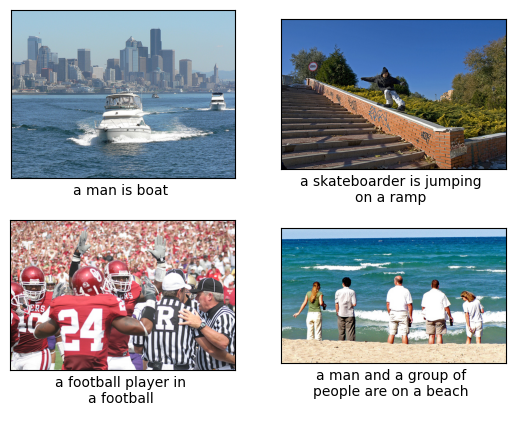
\includegraphics[width=.9\linewidth]{results/vit_transformer}
    \caption{Przykładowe obrazy wraz z podpisami wygenerowanymi przez architekturę wykorzystującą transformer wizyjny wraz z klasycznym transformerem. Opracowanie własne.}
    \label{fig:results-vit-transformer}
\end{figure}
\noindent Można zaobserwować, iż wygenerowane podpisy są o wiele dłuższe niż w porównaniu do architektury VIT i RNN, jednakże brakuje im logicznej spójności. W dużej mierze są one bez sensu, ale zawarte w nich rzeczowniki w większości odnoszą się do faktycznych obiektów znajdujących się na zdjęciach. Jest to dosyć logiczne ze względu na wykorzystanie wstępnie wyuczonych modułów kodujących, które były trenowane na zbiorze danych przeznaczonym do zadań klasyfikacyjnych. Wskazuje to na poprawne rozpoznawanie obiektów znajdujących się na obrazie, jednakże architektura nie potrafi ich połączyć w logiczną całości, za co odpowiedzialny jest moduł dekodujący generujący sekwencję. Mimo wykorzystania zaawansowanego modułu dekodującego, jakim jest transformer, jego danymi wejściowymi cały czas jest pojedynczy wektor reprezentujący obraz. Natomiast podpisy wygenerowane przez sieć GIT, widoczne na rysunku \ref{fig:results-git}, są o wiele bardziej zadowalające, tworzą one zrozumiałe zdania i można zauważyć w nich identyfikacje odpowiednich relacji pomiędzy obiektami znajdującymi się na zdjęciach.
\begin{figure}[H]
    \centering
    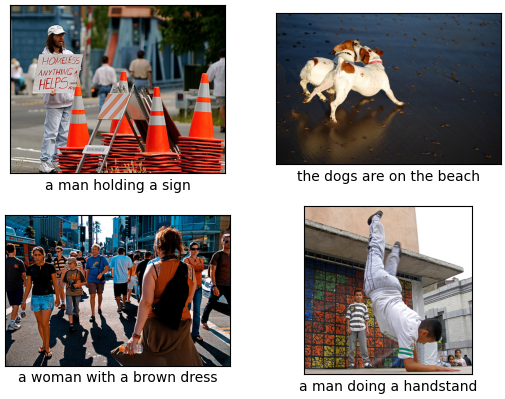
\includegraphics[width=.9\linewidth]{results/git_results}
    \caption{Przykładowe obrazy wraz z podpisami wygenerowanymi przez architekturę GIT. Opracowanie własne.}
    \label{fig:results-git}
\end{figure}
\noindent Tak dobry wynik w porównaniu do pozostałych architektur pokazuje duży wpływ modułu dekodującego na ostateczny rezultat oraz możliwości analizowania obrazu jako całą sekwencję, a nie tylko jako pojedynczy element początkowy. W przypadku tejże sieci warto również przypomnieć, iż w ramach testów wykorzystany został wcześniej wytrenowany model na zbiorze MS COCO, który nie był dostrojony do zbioru Flickr. Niestety tak dobra skuteczność oraz duży potencjał wiążą się z bardzo dużym zapotrzebowaniem na zasoby komputerowe. Wykorzystanie tego rozwiązania zajmuje bardzo dużo czasu i ze względu na ogromną liczbę parametrów nie jest możliwe jego użycie przy pomocy mniejszych kart graficznych, co znacząco wpływa na czas przetwarzania. W przypadku wykorzystania modelu wstępnie wyuczonego takie ograniczenia mogą nie być dużą przeszkodą, ale na pewno korzystając z modelu bez wstępnych wartości parametrów architektury, otrzymanie tak dobrego wyniku może okazać się nieosiągalne ze względu na ograniczenia zasobów komputerowych, czasowych lub budżetowych.

Warto również zwrócić uwagę na wyniki architektury wykorzystującej splotową sieć AlexNet. Rysunek \ref{fig:metrics-transformer} przedstawia wartości metryk wszystkich modułów kodujących w połączeniu z transformerem jako modułem dekodującym. Można na nim zauważyć bardzo dobry wynik w porównaniu do pozostałych architektur.
\begin{figure}[H]
    \centering
    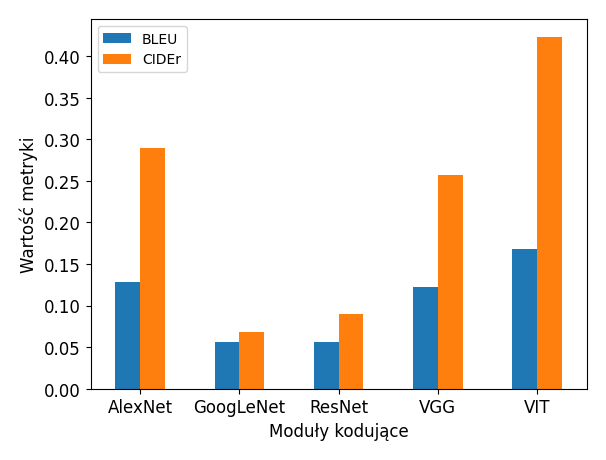
\includegraphics[width=.9\linewidth]{metrics/transformer_metrics}
    \caption{Wartości metryk BLEU oraz CIDEr dla poszczególnych modułów kodujących połączonych z transformerem jako modułem dekodującym. Opracowanie własne.}
    \label{fig:metrics-transformer}
\end{figure}
\noindent Sieć AlexNet ustąpiła jedynie miejsca architekturze GIT oraz kombinacjom modułów wykorzystujących transformer wizyjny. Wynika to z faktu, iż posiadała ona największą ostatnią warstwę w swojej architekturze. Zawierała ona ponad 4 tysiące parametrów -- GoogLeNet, ResNet posiadały ich zdecydowanie mniej, ponieważ odpowiednio: 1024 oraz 2048. Przykładowe podpisy wygenerowane przez architekturę AlexNet wraz z transformerem zostały przedstawione na rysunku \ref{fig:results-alexnet-transformer}. Są one dosyć podobne jakościowo do tych otrzymanych przy pomocy VIT.
\begin{figure}[H]
    \centering
    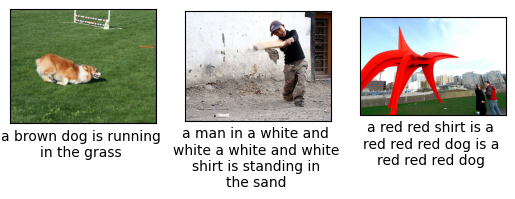
\includegraphics[width=.9\linewidth]{results/alexnet_transformer}
    \caption{Przykładowe obraz wraz z podpisami wygenerowanymi przez architekturę wykorzystującą transformer wizyjny wraz z siecią RNN. Opracowanie własne.}
    \label{fig:results-alexnet-transformer}
\end{figure}
\noindent Zaskakujący jest słabszy wynik architektury VGG, która posiadała taką samą liczbę parametrów jak AlexNet, a mimo wszystko okazała się mniej skuteczna w przypadku obu metryk. Ponownie można zwrócić uwagę na bardzo duży wpływ w analizowaniu obrazu poprzez wykorzystanie transformera wizyjnego, ponieważ pomimo posiadania najmniejszej liczby parametrów -- jedynie 768 -- architektury go wykorzystujące osiągnęły zdecydowanie najlepsze wyniki. Nie można jednocześnie zapomnieć o bardzo dużym wpływie liczby parametrów na czas potrzebny do wyuczenia danych architektur, które można zaobserwować na rysunku \ref{fig:timings-training-decoders-nvidia} dla karty graficznej Nvidia T4.
\begin{figure}[H]
    \centering
    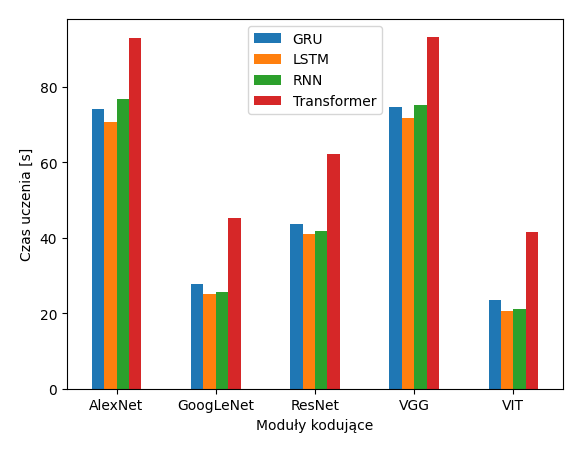
\includegraphics[width=.95\linewidth]{timings/timings_training_decoders_nvidia}
    \caption{Czas przetwarzania jednej epoki treningowej przy użyciu kart graficznej Nvidia T4 dla poszczególnych modułów dekodujących wykorzystujących wstępnie wyuczone moduły kodujące. Opracowanie własne.}
    \label{fig:timings-training-decoders-nvidia}
\end{figure}
\noindent Widoczny jest bezpośredni wpływ liczby parametrów modułów kodujących na czas przetwarzania. Jest to przewidywalnym wynikiem, ponieważ w przypadku większej ilości danych, sieć rekurencyjna musi przetworzyć ich stosunkowo więcej. Interesującym jest fakt, iż nie miało to bezpośredniego przełożenia na lepsze wyniki. Pokazuje to, iż bardzo istotne jest przeanalizowanie obrazu w odpowiedni sposób i najpewniej zwiększenie liczby parametrów w modułach kodujących miałoby w pewnym stopniu wpływ na poprawę skuteczności generowania podpisów, ale porównując różnice w przypadku takich sieci jak GoogLeNet, ResNet, VGG nie są one drastyczne. Warte zweryfikowania na pewno byłoby zwiększenie tejże ilości w przypadku transformera wizyjnego.
\subsection{Skuteczność architektury wykorzystującej zaproponowane połączenie}
Skuteczność rozwiązania wykorzystującego dane pochodzące z pośrednich warstw splotowych została przedstawiona na rysunku \ref{fig:metrics-modified}.
\begin{figure}[H]
    \centering
    \begin{subfigure}{.5\textwidth}
        \centering
        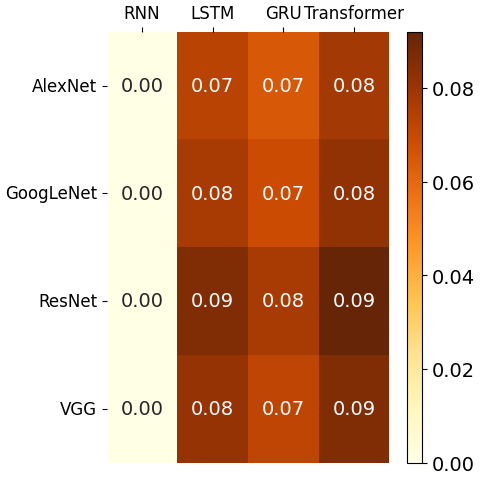
\includegraphics[width=.95\linewidth]{metrics/metrics_modified/BLEU}
        \caption{Wartości metryki BLEU}
        \label{fig:bleu-modified}
    \end{subfigure}%
    \centering
    \begin{subfigure}{.5\textwidth}
        \centering
        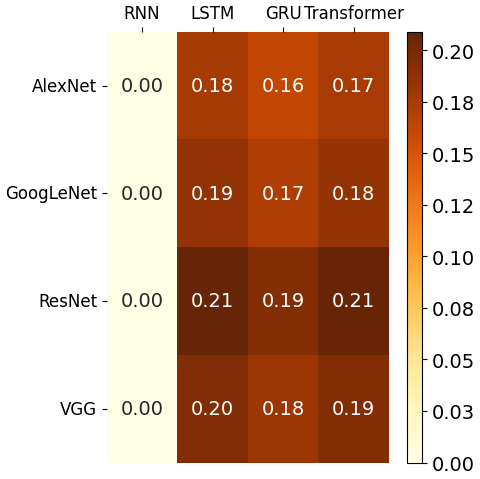
\includegraphics[width=.95\linewidth]{metrics/metrics_modified/CIDEr}
        \caption{Wartości metryki CIDEr}
        \label{fig:cider-modified}
    \end{subfigure}%
    \caption{Wartości metryk BLEU oraz CIDEr dla poszczególnych kombinacji modułów kodujących i dekodujących wykorzystujących zaproponowane połączenie. Opracowanie własne}
    \label{fig:metrics-modified}
\end{figure}
\noindent Ponownie można zauważyć, iż sieć RNN nie poradziła sobie z tym zadaniem i nie osiągnęła sensownych rezultatów -- dla każdej architektury splotowej wartość metryk wyniosła zero. W przypadku pozostałych modułów dekodujących otrzymane wyniki są do siebie zbliżone. Wyniki poszczególnych sieci splotowych są na bardzo zbliżonym poziomie, w przeciwieństwie do architektury z klasycznym połączeniem. Taki stan rzeczy wynika z faktu, iż wektor wyjściowy każdego modułu kodującego był takiego samego rozmiaru -- w przypadku architektury klasycznego połączenia wektory te różniły się rozmiarem, co miało bezpośredni wpływ na skuteczność danej architektury.

Na podstawie krzywych funkcji straty można zauważyć, iż w przypadku wykorzystania danych z warstw splotowych różnice pomiędzy wartościami zbioru walidacyjnego i treningowego są znacznie większe niż w przypadku klasycznego połączenia modułów, co można zaobserwować na rysunku \ref{fig:training-alexnet-gru-modified}, który przedstawia dane treningowe architektury składającej się z sieci AlexNet oraz GRU.
\begin{figure}[H]
    \centering
    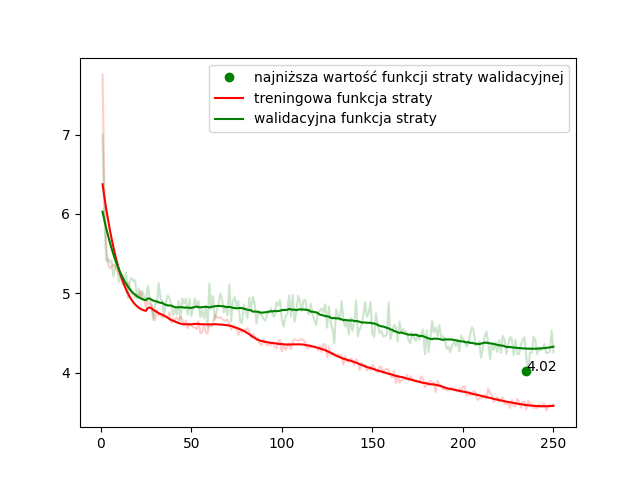
\includegraphics[width=.95\linewidth]{training/alexnet_gru_modified}
    \caption{Wykres wartości funkcji straty treningowej oraz walidacyjnej dla architektury składającej się z sieci AlexNet i GRU. Opracowanie własne.}
    \label{fig:training-alexnet-gru-modified}
\end{figure}
\noindent Mimo iż najlepsza wartość funkcji straty została osiągnięta przy końcu treningu, to już od połowy wartość walidacyjna nie spadała w takim samym tempie, co wartość funkcji straty na zbiorze treningowym. Może to świadczyć o zbyt małej generalizacji danych wejściowych. Można wysunąć wniosek, iż wykorzystywanie danych z warstw splotowych nie jest tak efektywne, ponieważ są to dane zbyt ogólne niezawierające kluczowych informacji o charakterystyce obrazu.
\subsection{Porównanie z innymi rozwiązaniami}
Najlepszą z architektur łączących bezpośrednio moduły kodujące i dekodujące okazało się połączenie transformera wizyjnego wraz z klasycznym transformerem, które wykorzystywało proste połączenie modułów. W przypadku połączenie uwzględniającego dane z warstw splotowych najlepszym rozwiązaniem okazało się połączeniem sieci ResNet oraz Transformera, jednakże metryki przez nie otrzymane były prawie dwukrotnie mniejsze niż wcześniej wspomniane rozwiązanie. Mimo to wartości metryk otrzymane przy pomocy tego rozwiązania mocno odstają od tych otrzymanych przy pomocy dedykowanych rozwiązań takich jak GIT oraz OFA, co zostało przedstawione w tabeli \ref{tab:comparison}. W przypadku rozwiązania GIT oraz OFA zostały tam umieszczone wyniki podane bezpośrednio przez autorów, jak również te otrzymane przy pomocy udostępnionych wstępnie wyuczonych modeli.
\begin{table}[H]
    \centering
    \caption{Porównanie skuteczności rozwiązania wykorzystującego VIT oraz transformera wizyjnego z innymi rozwiązaniami.}
    \label{tab:comparison}
    \begin{tabular}{|l|l|l|l|l|}
        \hline
        \textbf{Rozwiązanie} & \textbf{BLEU} & \textbf{METEOR} & \textbf{CIDEr} & \textbf{SPICE} \\ \hline
        VIT + Transformer    & 0,17          & 0,18            & 0,42           & 0,10           \\ \hline
        GIT (test)           & 0,19          & 0,17            & 0,58           & 0,13           \\ \hline
        GIT (artykuł)        & 0,40          & 0,30            & 1,31           & 0,23           \\ \hline
        OFA (test)           & 0,33          & 0,28            & 1,03           & 0,21           \\ \hline
        OFA  (artykuł)       & 0,43          & 0,32            & 1,45           & 0,25           \\ \hline
    \end{tabular}
\end{table}
\noindent Wartości metryk otrzymane dla architektury GIT w przypadku BLEU oraz METEOR są nieznacznie wyższe od rozwiązania VIT + Transformer. W przypadku metryk CIDEr i SPICE różnice są bardziej zauważalne, co może świadczyć o lepszej zdolności GIT do zachowania sensu i semantyki w generowanych podpisach. Jednakże porównując wyniki GIT z tymi podanymi bezpośrednio przez autorów architektury, zauważalne są znaczne różnice. Wartości wszystkich metryk dla testowanego wariantu są prawie dwukrotnie mniejsze niż te, które podali autorzy. Takie rozbieżności mogą wskazywać na słabą zdolność architektury do generalizacji na różne zbiory danych lub specyficzne warunki testowe. W przypadku architektury OFA, różnice między wartościami otrzymanymi w badaniach a tymi zawartymi w artykule są niewielkie. Wartości wszystkich metryk podane przez autorów są większe o kilka setnych, co sugeruje, że OFA utrzymuje stabilność wyników i skuteczność w różnych kontekstach. Może to wskazywać na lepszą generalizację i niezawodność architektury OFA w porównaniu do GIT, która również osiągnęła największe wartości w przypadku wszystkich podanych metryk.

\newpage % Rozdziały zaczynamy od nowej strony.
\section{Wnioski}
Najlepszym rozwiązaniem spośród wszelkich kombinacji modułów kodujących oraz dekodujących okazało się najbardziej zaawansowane połączenie, czyli transformer wizyjny wraz z klasycznym transformerem. Niestety takie rozwiązanie i tak odstaje od kompleksowych architektur stworzonych z myślą o generowaniu podpisów do obrazów, takich jak GIT i OFA. O wiele lepsza skuteczność tychże rozwiązań jednocześnie wiąże się z o wiele większymi wymaganiami sprzętowymi, które graniczą z możliwością ich wykorzystania. Szczególnie dotkliwe jest wymaganie alokacji dużej ilości pamięci, co skutkuje brakiem możliwości wykorzystania mniej zaawansowanych wersji jednostek GPU. Jest to główne ograniczenie, ponieważ w przypadku sieci, które były w stanie zostać uruchomione za pomocą mniejszej karty graficznej zostały przetworzone w podobnym czasie do tego przy wykorzystaniu znacznie bardziej zaawansowanej jednostki GPU. W przypadku dedykowanych architektur zarówno czas uczenia, jak i generowania podpisów jest znacząco większy niż w przypadku wykorzystywania mniej złożonych sieci. Pokazuje to, iż rozwój sztucznej inteligencji kieruje się w stronę coraz bardziej rozbudowanych i obciążających rozwiązań. Otrzymanie wyników bez wykorzystywania wstępnie wyuczonych modeli staje się coraz trudniejsze ze względu na potrzebę posiadania wielkiego zbioru danych oraz zasobów obliczeniowych. W przypadku architektury GIT czy OFA warto również pamiętać, że wstępnie wyuczone modele nie rozwiązują problemu późniejszych wymagań obliczeniowych potrzebnych w trakcie docelowego generowania podpisów. Jednoznacznie można stwierdzić, iż podstawowa sieć rekurencyjna nie jest w stanie sprostać zadaniu generowania podpisów do obrazów, a jej bardziej zaawansowani następcy jak LSTM czy GRU są o wiele lepszym wyborem. W przypadku sieci splotowych wybór najlepszego rozwiązania nie jest tak oczywisty. Wraz z lepszą skutecznością rosną wymagania sprzętowe. Tak duże wymagania obliczeniowe, jakie występują w procesie uczenia maszynowego, wywierają znaczący wpływ na czas potrzebny na wyuczenie modelu, co może stanowić jedno z kluczowych ograniczeń w dalszym rozwoju sztucznej inteligencji. Proces szkolenia modeli maszynowych wymaga ogromnych nakładów czasu zarówno na przetwarzanie, jak i adaptację do coraz bardziej rosnących zbiorów danych. Model uczenia maszynowego musi być zdolny do efektywnego przetwarzania ogromnych ilości informacji, a jednocześnie szybko dostosowywać się do zmieniających się warunków. Owa potrzeba adaptacji jest szczególnie ważna w kontekście dynamicznie rozwijającego się świata, gdzie ilość generowanych danych z dnia na dzień znacząco rośnie. Dzięki temu modele mogą lepiej reprezentować rzeczywistość i dostosowywać się do zmieniających się wzorców. Otrzymane wyniki w kwestii czasu potrzebnego na przetwarzanie architektur sieci neuronowych, jak również wymagania sprzętowe pokazują, iż może stanowić to duże ograniczenie w dalszym rozwoju tychże rozwiązań.
\subsection{Perspektywy rozwoju}
Ze względu na ograniczenia czasowe nie było możliwe zweryfikowanie, jak duży wpływ ma równoczesne trenowanie modułu kodującego wraz z modułem dekodującym na skuteczność otrzymanych rozwiązań. Można przypuszczać, iż skuteczność w pewnym stopniu by wzrosła, ale są to jedynie domysły, które warte są weryfikacji. Być może wartym zweryfikowania byłyby również inne architektury modułów kodujących i dekodujących stworzone z myślą o większej wydajności.


%--------------------------------------------
% Literatura
%--------------------------------------------
\cleardoublepage % Zaczynamy od nieparzystej strony
\printbibliography

%--------------------------------------------
% Spisy (opcjonalne)
%--------------------------------------------
\newpage
\pagestyle{plain}

% Wykaz symboli i skrótów.
% Pamiętaj, żeby posortować symbole alfabetycznie
% we własnym zakresie. Ponieważ mało kto używa takiego wykazu,
% uznałem, że robienie automatycznie sortowanej listy
% na poziomie LaTeXa to za duży overkill.
% Makro \acronymlist generuje właściwy tytuł sekcji,
% w zależności od języka.
% Makro \acronym dodaje skrót/symbol do listy,
% zapewniając podstawowe formatowanie.
% //AB
% \vspace{0.8cm}
% \acronymlist
% % TODO uzupełnić
% \acronym{CNN}{Splotowa sieć neuronowa}
% \acronym{RNN}{Rekurencyjna sieć neuronowa}
% \acronym{LSTM}{Long short-term memory}
% \acronym{GRU}{Gated recurrent unit}

\listoffigurestoc     % Spis rysunków.
% \vspace{1cm}          % vertical space
% \listoftablestoc      % Spis tabel.
% \vspace{1cm}          % vertical space
% \listofappendicestoc  % Spis załączników

% Używając powyższych spisów jako szablonu,
% możesz tu dodać swój własny wykaz bądź listę,
% np. spis algorytmów.

\end{document} % Dobranoc.
